% !TEX root=../dummy/dummy-05.tex

\section{第 \ref{sec.5.title} 章补充内容}

\subsection{HR46 与 T144 数据集分子结构}

\begin{figure}[H]
    \centering
    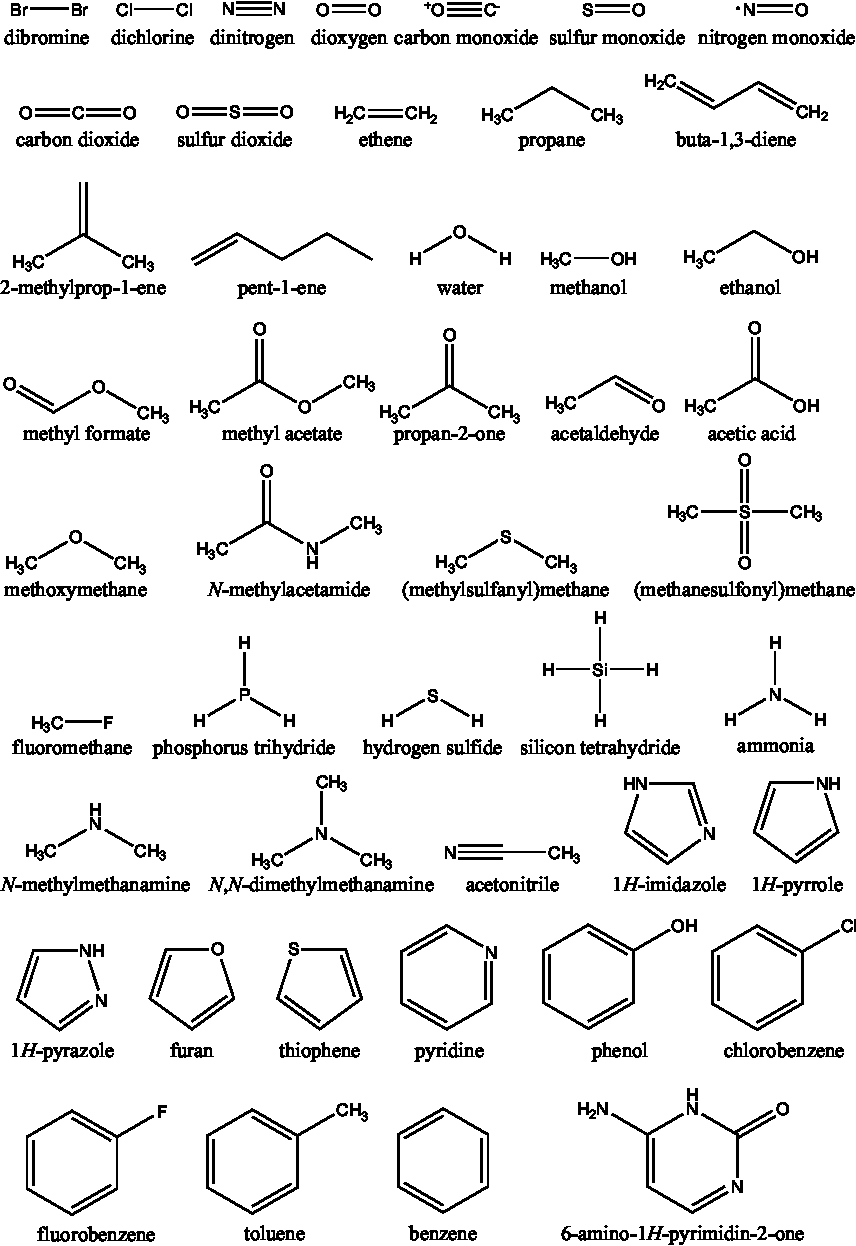
\includegraphics[width=0.85\textwidth]{assets/fig-s1.pdf}
    \caption[HR46 数据集分子结构]{HR46 数据集分子结构。}
    \label{fig.fig-s1}
\end{figure}

\begin{figure}[!p]
    \centering
    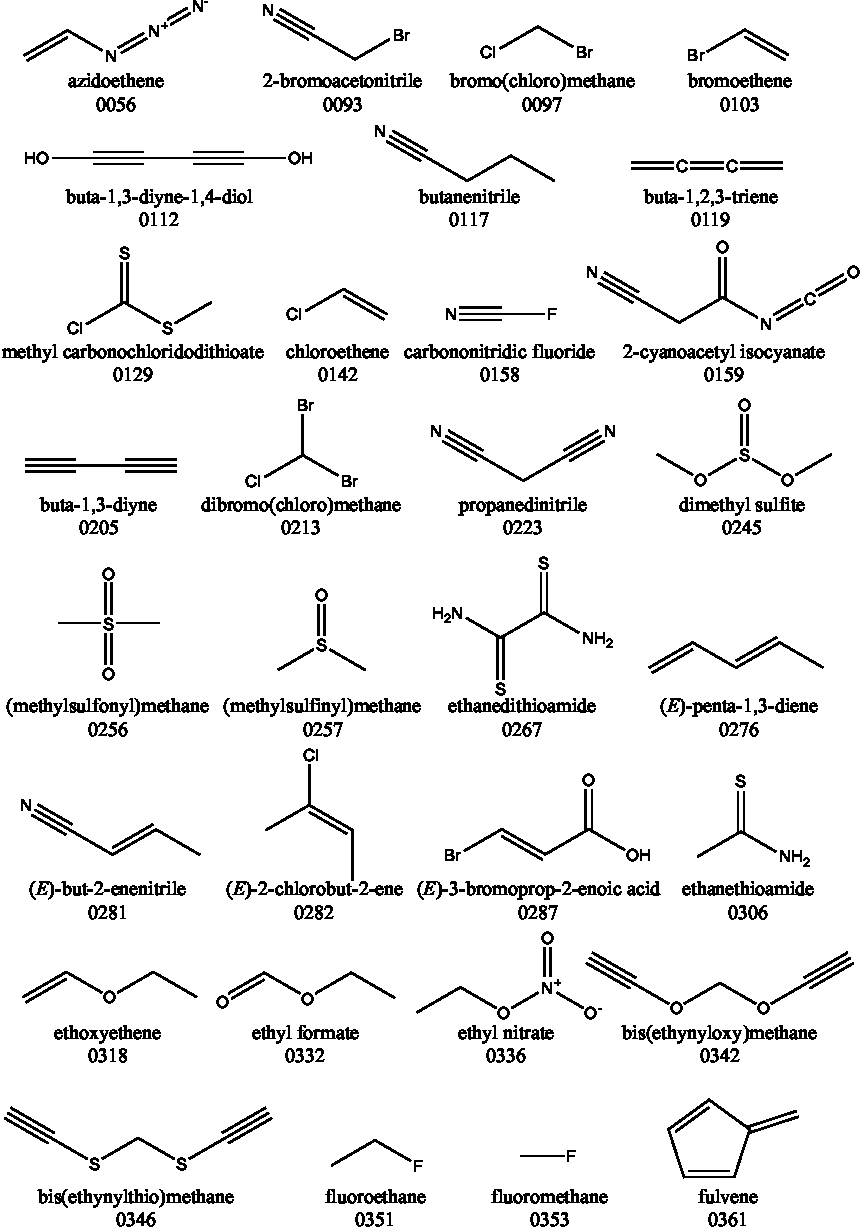
\includegraphics[width=0.85\textwidth]{assets/fig-s2-1.pdf}
    \caption[T144 数据集分子结构]{T144 数据集分子结构。}
    \label{fig.fig-s2-1}
\end{figure}

\setcounter{figure}{\value{figure} - 1}

\begin{figure}[!p]
    \centering
    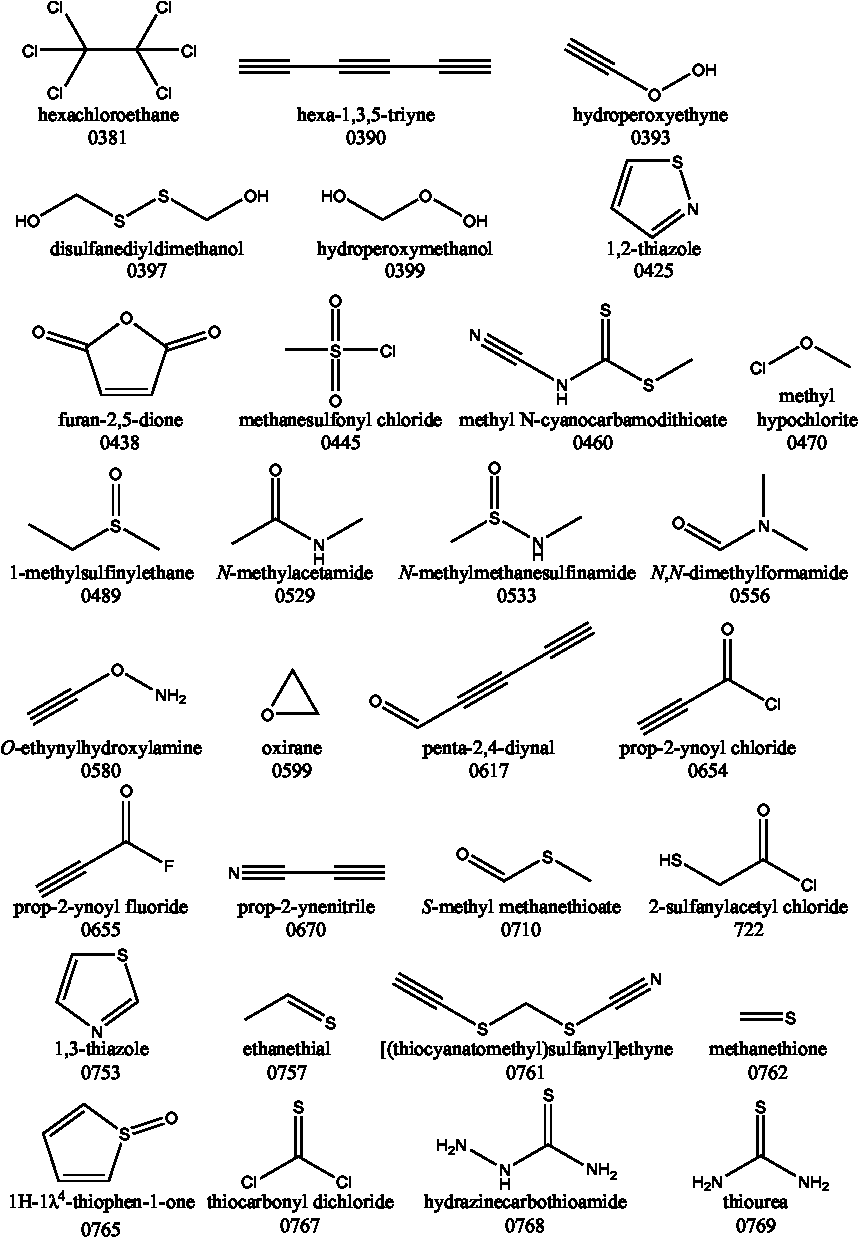
\includegraphics[width=0.85\textwidth]{assets/fig-s2-2.pdf}
    \caption[]{(续图)}
    \label{fig.fig-s2-2}
\end{figure}

\setcounter{figure}{\value{figure} - 1}

\begin{figure}[!p]
    \centering
    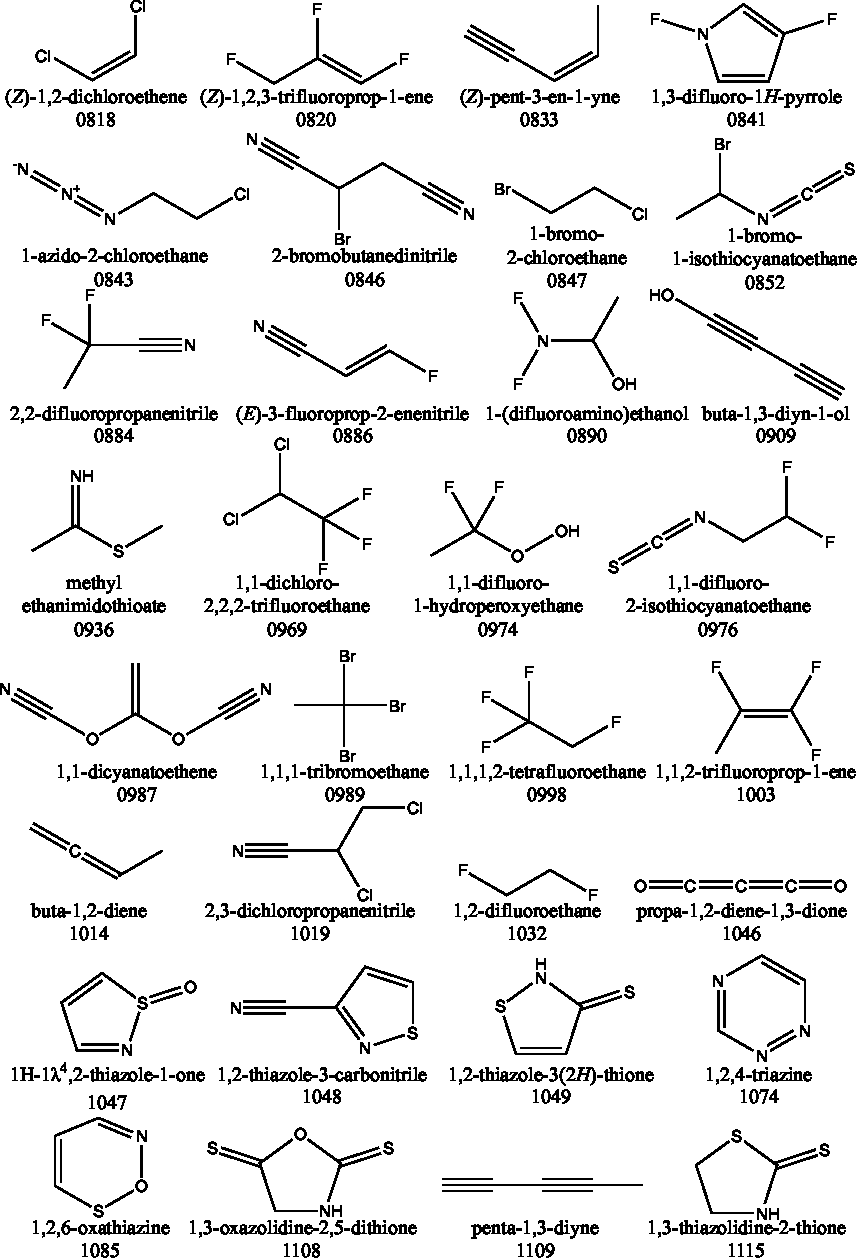
\includegraphics[width=0.85\textwidth]{assets/fig-s2-3.pdf}
    \caption[]{(续图)}
    \label{fig.fig-s2-3}
\end{figure}

\setcounter{figure}{\value{figure} - 1}

\begin{figure}[!p]
    \centering
    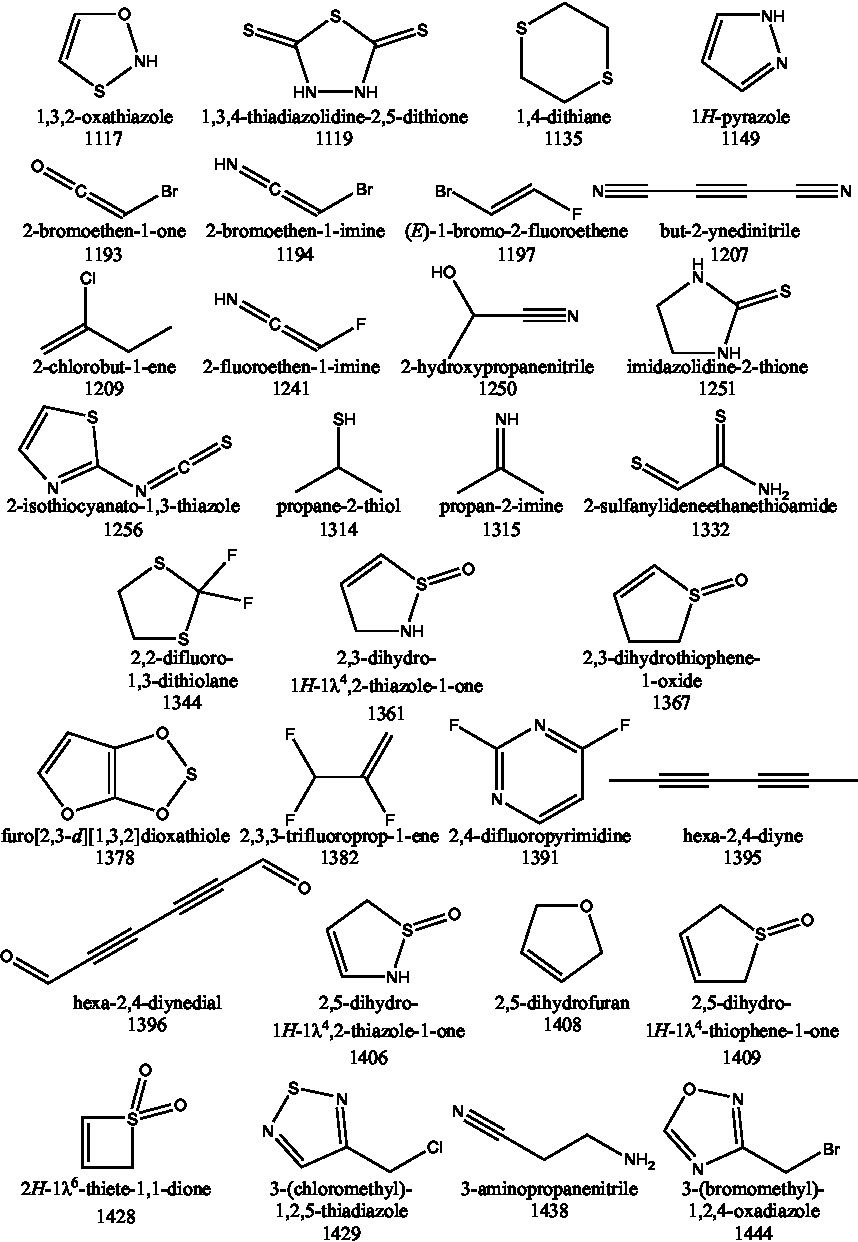
\includegraphics[width=0.85\textwidth]{assets/fig-s2-4.pdf}
    \caption[]{(续图)}
    \label{fig.fig-s2-4}
\end{figure}

\setcounter{figure}{\value{figure} - 1}

\begin{figure}[!p]
    \centering
    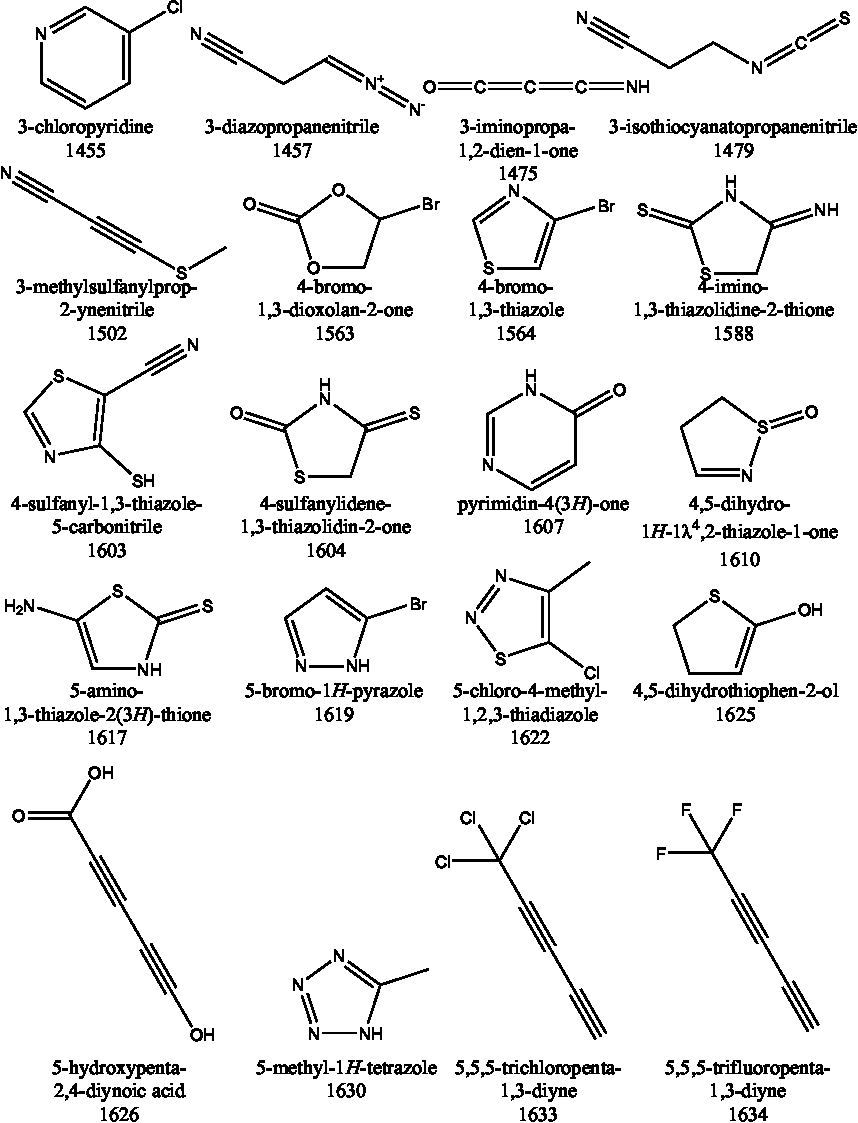
\includegraphics[width=0.85\textwidth]{assets/fig-s2-5.pdf}
    \caption[]{(续图)}
    \label{fig.fig-s2-5}
\end{figure}

\clearpage

\subsection{体系名称的更改}
\label{sec.T145-HR46-name-change}

本工作会对原先 T144 与 HR46 数据集的化合物名称作一定更改。我们尽量依照 IUPAC 推荐命名规则 (PIN) 进行命名\cite{Favre-Powell.RSC.2013}。举例而言,“acetone”(丙酮) 将被命名为“propane-2-one”(丙-2-酮)。这类名称更改是平凡的。

HR46 原文献\cite{Hickey-Rowley.JPCA.2014}中,正文中名称为“thymine”的分子应命名为“cytosine”(胞嘧啶,或 PIN 命名 6-amino-1\textit{H}-pyrimidin-2-one)。其补充信息中的命名是正确的。

T144 数据集中,我们依据 TABS 数据库所提供的分子坐标文件,对下述 4 个分子的名称作勘定,并示于表 \ref{tab.T144-name-errata}。

\begin{table}[!ht]
\centering
\caption[T144 数据集分子名称勘定]{T144 数据集分子名称勘定。}
\label{tab.T144-name-errata}
\widetabular{
    \begin{tabular}{lll}
    \toprule
    编号   & TABS 数据集化合物名称 & 修订化合物名称 \\ \midrule
    0129 & carbonochloridodithioic   acid & methyl   carbonochloridodithioate \\
    0399 & hydroxymethylperoxide          & hydroperoxymethanol               \\
    1193 & 2-bromoethanone                & 2-bromoethen-1-one                \\
    1630 & 5-methyl-2\textit{H}-tetrazole          & 5-methyl-1\textit{H}-tetrazole             \\ \bottomrule
    \end{tabular}
}{}
\end{table}

\subsection{CCSD 方法下不同 FPA 模型之间的相对误差}

下述的表 \ref{tab.5.s5} 与表 \ref{tab.5.s6} 整理了 CCSD 计算数据,它是针对正文 \ref{tab.5.5} 与表 \ref{tab.5.6} 整理的 CCSD(T) 数据的补充。

\begin{table}[!ht]
\centering
\caption[HR46 与 T144 子集 $\symup{\Delta} \tilde \alpha_\textsf{CCSD}$ 在不同 FPA 模型下 RelRMSD]{HR46 与 T144 子集下同性极化率 $\symup{\Delta} \tilde \alpha_\textsf{CCSD}$ 在不同 FPA 模型下的相对方均根误差\textrm{\textsuperscript{\emph{a}}}。}
\label{tab.5.s5}
\widetabular{
    \begin{tabular}{ccccc}
    \toprule
    数据集 & 数据子集 & Scheme & Reference & RelRMSD / \% \\ \midrule
    HR46    & I      & FPA-aV[DT]Z & FPA-aV[Q5]Z & 0.163 \\
            & I      & FPA-aV[TQ]Z & FPA-aV[Q5]Z & 0.151 \\
            & II     & FPA-aV[DT]Z & FPA-aV[TQ]Z & 0.084 \\
    T144    & I      & FPA-aV[DT]Z & FPA-aV[TQ]Z & 0.140 \\ \bottomrule
    \end{tabular}
}{
    \item[a] 相对误差以 $\text{RelRMSD} (\tilde \alpha_{\textsf{CCSD}/\text{Scheme}}, \tilde \alpha_{\textsf{CCSD}/\text{Reference}})$ 呈现。
}
\end{table}

\begin{table}[!ht]
\centering
\caption[HR46 与 T144 子集 $\symup{\Delta} \tilde \gamma_\textsf{CCSD}$ 在不同 FPA 模型下 RelRMSD]{HR46 与 T144 子集下异性极化率 $\symup{\Delta} \tilde \gamma_\textsf{CCSD}$ 在不同 FPA 模型下的相对方均根误差\textrm{\textsuperscript{\emph{a}}}。}
\label{tab.5.s6}
\widetabular{
    \begin{tabular}{ccccc}
    \toprule
    数据集 & 数据子集 & Scheme & Reference & RelRMSD / \% \\ \midrule
    HR46    &  I & FPA-aV[DT]Z & FPA-aV[Q5]Z & 0.299 \\
            &  I & FPA-aV[TQ]Z & FPA-aV[Q5]Z & 0.335 \\
            & II & FPA-aV[DT]Z & FPA-aV[TQ]Z & 0.208 \\
    T144    &  I & FPA-aV[DT]Z & FPA-aV[TQ]Z & 0.214 \\ \bottomrule
    \end{tabular}
}{
    \item[a] 相对误差以 $\text{RelRMSD} (\tilde \gamma_{\textsf{CCSD}/\text{Scheme}}, \tilde \gamma_{\textsf{CCSD}/\text{Reference}})$ 呈现。统计误差时,仅考虑 $\gamma_{\textsf{CCSD(T)}}$ 大于 0.5 $\text{\AA}{}^{3}$ 的体系。关于具体被考虑的体系,参考表 \ref{tab.5.6}。
}
\end{table}

\subsection{对有限差分误差的分析}
\label{sec.5.s9}

对同性极化率 $\alpha$ 所作的因有限差分而导致误差的分析列于表 \ref{tab.5.s8}。作为参照的数值是解析梯度所计算得到的极化率。我们假定对异性极化率 $\gamma$ 应有类似的结论。在该分析中,我们将使用两种自洽场收敛判据。需要指出,解析梯度极化率的精度也受机器精度、自洽场收敛精度与 CP-HF 方程收敛精度等要素影响;但在这段分析中,我们假定这些影响要素可以忽略不计。

\begin{table}[ht]
\centering
\caption[HR45 数据集同性极化率因数值导数而起的 RelRMSD]{HR45 数据集同性极化率因数值导数而起的相对方均差 (RelRMSD)\textrm{\textsuperscript{\emph{a}}}。}
\label{tab.5.s8}
\widetabular{
    \begin{tabular}{ccccccc}
    \toprule
    & \multicolumn{2}{c}{$\alpha_\textsf{MP2}$ / \%\tnote{b}} & \multicolumn{2}{c}{$\alpha_\textsf{HF}$ / \%\tnote{c}} & \multicolumn{2}{c}{$\symup{\Delta} \alpha_\textsf{(2)}$ / \%\tnote{d}} \\
    \cmidrule(lr){2-3} \cmidrule(lr){4-5} \cmidrule(lr){6-7}
    外场强度 $h$ / au & loose\tnote{e}         & tight\tnote{f}        & loose\tnote{e}        & tight\tnote{f}        & loose\tnote{e}         & tight\tnote{f}         \\
    \midrule
    0.0005            & 1.625          & 0.000         & 0.000         & 0.000         & 1.625          & 0.000          \\
    0.0010            & 0.395          & 0.002         & 0.001         & 0.001         & 0.395          & 0.001          \\
    0.0020            & 0.046          & 0.006         & 0.005         & 0.005         & 0.046          & 0.002          \\
    0.0040            & 0.031          & 0.025         & 0.019         & 0.019         & 0.020          & 0.008          \\
    0.0080            & 0.101          & 0.101         & 0.075         & 0.075         & 0.033          & 0.033          \\
    0.0160            & 0.415          & 0.415         & 0.309         & 0.309         & 0.138          & 0.138          \\
    \bottomrule
    \end{tabular}
}{
    \item[a] 该表格数据是通过 \textsc{PySCF} 结合扩展程序 \textsc{dh},以 aVTZ 级别基组计算,对 HR45 数据集 (除去了 \ce{^2NO} 分子的 HR46 数据集),在不同的自洽场收敛条件、以及不同的有限差分外场强度 $h$ 下所给出 (其意义在式 (\ref{eq.pol-findiff-alpha-def}, \ref{eq.pol-findiff-gamma-def}) 给出)。所有计算都使用 RI 近似,且 RI 辅助基选用 \textsc{PySCF} 默认的 ETB 给出。
    \item[b] $\alpha_\textsf{MP2}$ 的相对方均根误差是指 $\text{RelRMSD} (\tilde \alpha^\text{num}_\textsf{RI-MP2}, \tilde \alpha^\text{anal}_\textsf{RI-MP2})$。
    \item[c] $\alpha_\textsf{HF}$ 的相对方均根误差是指 $\text{RelRMSD} (\tilde \alpha^\text{num}_\textsf{RI-JK}, \tilde \alpha^\text{anal}_\textsf{RI-JK})$。
    \item[d] $\symup{\Delta} \alpha_\textsf{(2)}$ 的相对方均根误差是指 $\text{RelRMSD} (\symup{\Delta} \tilde \alpha^\text{num}_\textsf{RI-(2)}, \symup{\Delta} \tilde \alpha^\text{anal}_\textsf{RI-(2)}, \tilde \alpha^\text{anal}_\textsf{RI-MP2})$。
    \item[e] 宽松的 (loose) 收敛条件是指,在 \textsc{PySCF} 的两次相邻的自洽场迭代过程中,当达到能量阈值 (\texttt{conv\_tol}) $10^{-10}$ au 且达到轨道梯度阈值 (\texttt{conv\_tol\_grad}) $10^{-5}$ 时,则判定自洽场收敛。该表格所有数据都成功在 50 次自洽场迭代中以宽松条件收敛。该收敛条件亦用于正文中的所有解析极化率计算过程。
    \item[f] 严格的 (tight) 收敛条件是指,在 \textsc{PySCF} 的两次相邻的自洽场迭代过程中,当达到能量阈值 (\texttt{conv\_tol}) $10^{-13}$ au 且达到轨道梯度阈值 (\texttt{conv\_tol\_grad}) $10^{-10}$ 时、或自洽场已经进行了 50 次迭代,则不论是否真正地收敛而停止自洽场迭代。
}
\end{table}

我们看到对于 $\alpha_\textsf{HF}$,数值与解析导数之间的误差近乎完全来自于外加偶极电场强度 $h$;但对于 MP2 的相关贡献部分 $\symup{\Delta} \alpha_\textsf{(2)}$,若自洽场没有以严格的判标收敛,那么极化率的结果将会有比较显著的误差。

对于任何计算,特别是 post-SCF 方法的分子性质计算,自洽场的收敛当然是越精确、收敛判标越严格越好。但在现实的计算资源内、以及考虑到计算成本与精度需求的平衡,过分严格的自洽场并不一定划算、也不一定可以真的实现。考虑到我们对本工作的极化率参考值误差的预期是 0.5\% 以内;一方面,我们不希望在方法和基组误差之外,还有很大的有限差分误差;但另一方面,我们注意到在外加电场强度在 $h = 0.0040 \, \text{au}$ 时,在相对宽松的 (\textsc{PySCF} 默认的) 自洽场收敛判据下,$\alpha_\textsf{MP2}$ 的数值极化率与理论极化率的相对方均根误差仅有 0.031\%。据此我们推测,对于其他后自洽场方法 (譬如 CCSD(T)),对同性极化率 $\alpha$ 与异性极化率 $\gamma$,在自洽场收敛判据不低于 $10^{-10}$ au、对于更大基组且未引入 RI 近似的情形、以及对于其他数据集,若使用外加电场强度 $h = 0.0040 \, \text{au}$ 作数值差分,那么因差分而引入的误差大约在 0.05\% 的级别。这种程度的误差相比于实验精度的 0.5\% 误差,是完全可以忽略的。

\subsection{异性极化率 $\gamma$ 在不同基组下的绝对值方均根误差分析}

\begin{table}[!ht]
\centering
\caption[12 个自旋非极化小体系异性极化率 RMSD 误差]{12 个自旋非极化小体系异性极化率的绝对值方均根 (RMSD) 误差。该表格误差单位为 $\text{\AA}{}^{3}$。}
\label{tab.5.s7}
\widetabular{
    \begin{tabular}{cld{1.3}d{1.3}d{1.3}d{1.3}d{1.3}d{1.3}d{1.3}d{1.3}}
    \toprule
          &              & \multicolumn{4}{c}{7 个小体系\tnote{a}} & \multicolumn{4}{c}{5 个小体系\tnote{b}} \\
    \cmidrule(lr){3-6} \cmidrule(lr){7-10}
    基组基数 & 基组 &
    \multicolumn{1}{c}{$\tilde \gamma_\textsf{HF}$\tnote{c}}  &
    \multicolumn{1}{c}{$\symup{\Delta} \tilde \gamma_\textsf{(2)}$\tnote{c}}  &
    \multicolumn{1}{c}{$\symup{\Delta} \tilde \gamma_\textsf{D}$\tnote{c}} &
    \multicolumn{1}{c}{$\symup{\Delta} \tilde \gamma_\textsf{D(T)}$\tnote{c}} &
    \multicolumn{1}{c}{$\tilde \gamma_\textsf{HF}$\tnote{c}}  &
    \multicolumn{1}{c}{$\symup{\Delta} \tilde \gamma_\textsf{(2)}$\tnote{c}}  &
    \multicolumn{1}{c}{$\symup{\Delta} \tilde \gamma_\textsf{D}$\tnote{c}} &
    \multicolumn{1}{c}{$\symup{\Delta} \tilde \gamma_\textsf{D(T)}$\tnote{c}}
    \\ \midrule
    2-$\zeta$   & aVDZ         & 0.101  & 0.018  & 0.028 & 0.014 & 0.035  & 0.018  & 0.022 & 0.016 \\
          & aCVDZ        & 0.100  & 0.016  & 0.025 & 0.013 & 0.034  & 0.018  & 0.020 & 0.016 \\ \midrule
    3-$\zeta$   & aVTZ         & 0.028  & 0.010  & 0.011 & 0.006 & 0.012  & 0.016  & 0.008 & 0.006 \\
          & aCVTZ        & 0.018  & 0.006  & 0.008 & 0.006 & 0.011  & 0.014  & 0.007 & 0.006 \\
          & aV[DT]Z  &         & 0.013  & 0.004 & 0.003 &         & 0.020  & 0.004 & 0.004 \\
          & aCV[DT]Z &         & 0.008  & 0.004 & 0.004 &         & 0.017  & 0.005 & 0.005 \\ \midrule
    4-$\zeta$   & aVQZ         & 0.011  & 0.008  & 0.005 & 0.004 & 0.003  & 0.013  & 0.004 & 0.002 \\
          & aCVQZ        & 0.004  & 0.003  & 0.002 & 0.002 & 0.004  & 0.009  & 0.004 & 0.003 \\
          & aV[TQ]Z  &         & 0.008  & 0.005 & 0.005 &         & 0.010  & 0.003 & 0.002 \\
          & aCV[TQ]Z &         & 0.002  & 0.004 & 0.003 &         & 0.005  & 0.004 & 0.003 \\ \midrule
    5-$\zeta$   & aV5Z         & 0.003  & 0.003  & 0.002 & 0.002 & 0.000  & 0.007  & 0.002 & 0.001 \\
          & aCV5Z        & \multicolumn{1}{c}{0\tnote{d}} & 0.002  & 0.001 & 0.001 & \multicolumn{1}{c}{0\tnote{d}} & 0.004  & 0.002 & 0.001 \\
          & aV[Q5]Z  &         & 0.002  & 0.001 & 0.001 &         & 0.002  & 0.001 & 0.000 \\
          & aCV[Q5]Z &         & \multicolumn{1}{c}{0\tnote{d}} & \multicolumn{1}{c}{0\tnote{d}} & \multicolumn{1}{c}{0\tnote{d}} &         & \multicolumn{1}{c}{0\tnote{d}} & \multicolumn{1}{c}{0\tnote{d}} & \multicolumn{1}{c}{0\tnote{d}} \\ \bottomrule
    \end{tabular}
}{
    \item[a] 这 7 个小体系是 $\gamma_\textsf{CCSD(T)} > 0.5 \, \text{\AA}{}^3$ 的体系 (\ce{Cl2}, \ce{CO}, \ce{CO2}, \ce{FCN}, \ce{HCHS}, \ce{N2}, \ce{O2})。这些体系也是表 \ref{tab.5.3} 分析的体系。
    \item[b] 这 5 个小体系是 $\gamma_\textsf{CCSD(T)} < 0.5 \, \text{\AA}{}^3$ 的体系 (\ce{H2O}, \ce{H2S}, \ce{NH3}, \ce{PH3}, \ce{SiH4})。
    \item[c] 这些记号的定义参考表 \ref{tab.5.2} 与表 \ref{tab.5.3}。
    \item[d] 这些数值依据参考值的选取方式,从定义上是零。
}
\end{table}

在正文表 \ref{tab.5.3} 中,自旋非极化的异性极化率的分析仅限于 7 个分子,而 5 个分子因其 $\gamma_\textsf{CCSD(T)}$ 过小、以至于不适合使用相对误差判标分析。为对所有这 12 个分子进行合理的分析,我们在表 \ref{tab.5.s7} 中补充了以异性极化率绝对值的方均根误差 (RMSD) 为量标的分析。根据表格中的数据,我们认为,这 5 个 $\gamma_\textsf{CCSD(T)}$ 较小体系的基组收敛性误差与 7 个 $\gamma_\textsf{CCSD(T)}$ 较大体系相当。但若将这 5 个 $\gamma_\textsf{CCSD(T)}$ 较小体系引入表 \ref{tab.5.3},则会产生非常严重与异常的误差。我们相信,表 \ref{tab.5.3} 排除这 5 个体系,不会破坏对该表格的分析结论的合理性。

\subsection{$\symup{\Delta} \alpha_\textsf{D(T)}$ 对体系 \ce{^3O2}, \ce{^3SO}, \ce{Cl2} 计算结果的基组收敛趋势}
\label{sec.5.s4}

这里的讨论是对正文表 \ref{tab.5.2} 中异常数据的分析。需要注意本小节与下一小节对基组收敛性分析图片的纵坐标是对称对数坐标:当误差大于 0.1\% 或小于 -0.1\% 时选用对数坐标;当误差介于两者之间时选用线性坐标。对于特定基组,其相对误差是由下式所计算:
\begin{equation*}
    \frac{\symup{\Delta} \alpha_{\textsf{D(T)} / \text{basis}} - \symup{\Delta} \alpha_{\text{aCV[Q5]Z}}}{\alpha_{\textsf{CCSD(T)} / \text{ref}}}
\end{equation*}
图片中的叉形散点是 CBS 外推过程;图中的 CBS 外推将绘制在比原先基组基数 $\zeta$ 大 1 的位置上;即 [DT]Z 被看作是 QZ (4-$\zeta$) 级别、即 [TQ]Z 被看作是 5Z (5-$\zeta$) 级别、即 [Q5]Z 被看作是 6Z (6-$\zeta$) 级别。相对误差介于 -0.5\% 与 0.5\% 之间的部分以浅绿色背景展示。

\textbf{\ce{^3O2} 的基组收敛性。}收敛情况如图 \ref{fig.O2-iso} 所示。对于该体系,$\symup{\Delta} \alpha_\textsf{D(T)}$ 在 aCVDZ 上的表现比 aVDZ 要更好、但 aCVTZ 上的表现比 aVTZ 要差。因此,尽管 aCV[DT]Z 作为 CBS 外推,确实其效果比 aCVTZ 要好;但外推的进步相比于 aV[DT]Z 与 aVTZ 之间的差距,则要小许多。因此会出现更大的、核层矫正的基组外推 aCV[DT]Z 不如 aV[DT]Z 的情况。

\begin{figure}[!ht]
    \centering
    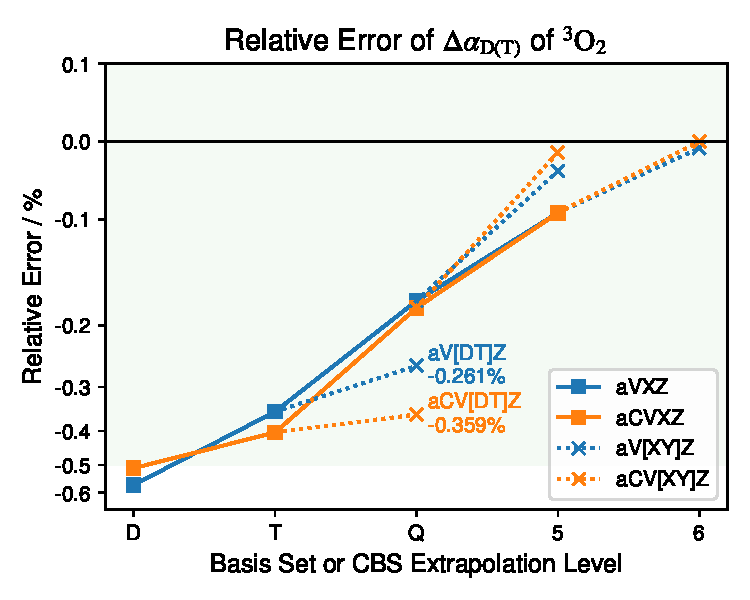
\includegraphics[width=0.5\textwidth]{assets/O2-iso.pdf}
    \caption[$\symup{\Delta} \alpha_\textsf{D(T)}$ 对体系 \ce{^3O2} 计算结果的基组收敛趋势]{$\symup{\Delta} \alpha_\textsf{D(T)}$ 对体系 \ce{^3O2} 计算结果的基组收敛趋势。}
    \label{fig.O2-iso}
\end{figure}

\textbf{\ce{^3SO} 的基组收敛性。}收敛情况如图 \ref{fig.SO-iso} 所示。对于该体系,我们能看到尽管更大的 aCVDZ 与 aCVTZ 基组本身的表现分别都要好于 aVDZ 与 aVTZ;但 aCV$X$Z 在该体系下收敛速度太快,因此 aCV[DT]Z 反而因为较为激进的 CBS 外推策略,而产生了较大的误差。相比之下,aV$X$Z 的基组收敛趋势与式 (\ref{eq.cbs.zeta3}) 较为接近,因此 aV[DT]Z 的结果很接近精确结果。

\begin{figure}[!ht]
    \centering
    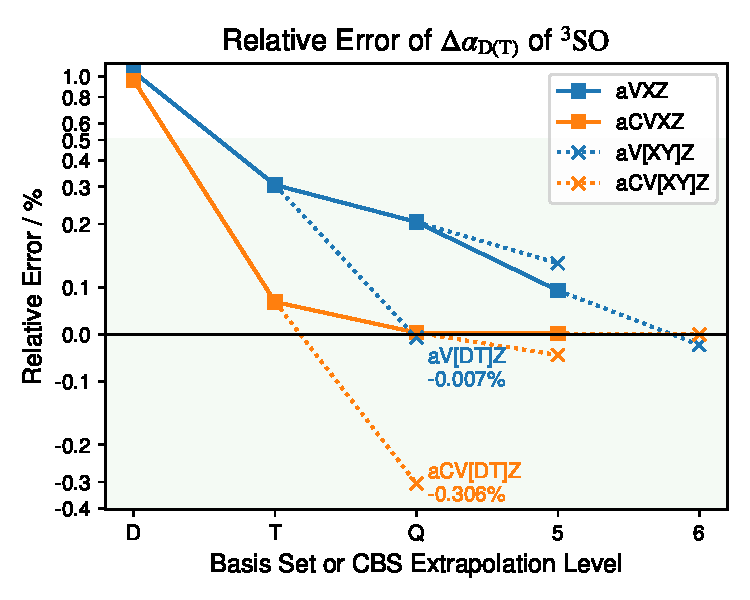
\includegraphics[width=0.5\textwidth]{assets/SO-iso.pdf}
    \caption[$\symup{\Delta} \alpha_\textsf{D(T)}$ 对体系 \ce{^3SO} 计算结果的基组收敛趋势]{$\symup{\Delta} \alpha_\textsf{D(T)}$ 对体系 \ce{^3SO} 计算结果的基组收敛趋势。}
    \label{fig.SO-iso}
\end{figure}

\textbf{\ce{Cl2} 的基组收敛性。}收敛情况如图 \ref{fig.Cl2-iso} 所示。该体系的情况与 \ce{^3SO} 有相似之处。其 aCV$X$Z 总体上比 aV$X$Z 的结果要更好,但由于收敛趋势与式 (\ref{eq.cbs.zeta3}) 有一定偏离,因此导致 aCV[TQ]Z 的 CBS 外推误差比 aV[TQ]Z 要更大,并且 aCV[TQ]Z 和 aV[TQ]Z 的误差要比代价更低的 aCV[DT]Z 和 aV[DT]Z 要更大。

\begin{figure}[!ht]
    \centering
    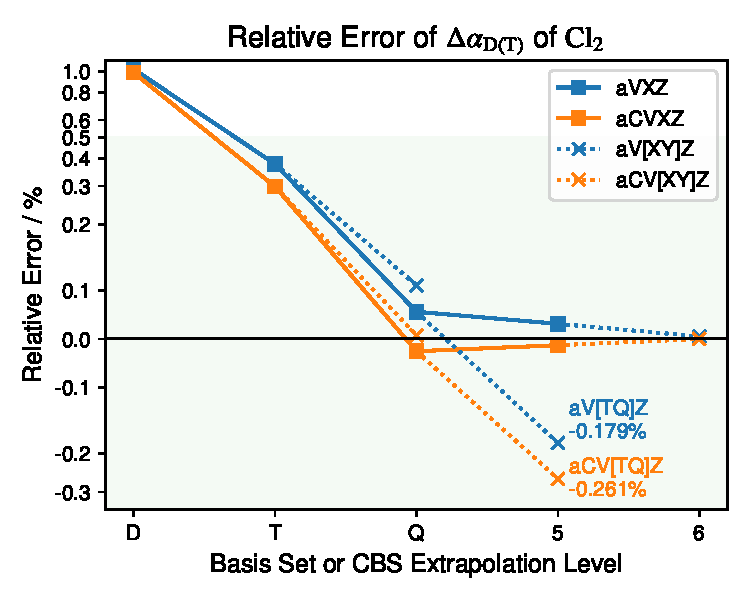
\includegraphics[width=0.5\textwidth]{assets/Cl2-iso.pdf}
    \caption[$\symup{\Delta} \alpha_\textsf{D(T)}$ 对体系 \ce{Cl2} 计算结果的基组收敛趋势]{$\symup{\Delta} \alpha_\textsf{D(T)}$ 对体系 \ce{Cl2} 计算结果的基组收敛趋势。}
    \label{fig.Cl2-iso}
\end{figure}

\subsection{$\symup{\Delta} \gamma_\textsf{D(T)}$ 对体系 \ce{^3O2}, \ce{^3SO}, \ce{HCHS}, \ce{Cl2} 计算结果的基组收敛趋势}
\label{sec.5.s5}

这里的讨论是对正文表 \ref{tab.5.3} 中异常数据的分析、以及作自旋非极化分子在异性极化率 $\gamma$ 下基组收敛情况的补充。

\textbf{\ce{^3O2} 的基组收敛性。}自旋极化的分子相比于自旋非极化的分子,在计算异性极化率 $\symup{\Delta} \gamma_\textsf{D(T)}$ 时,使用较小的基组或 CBS 外推模型,比起同性极化率 $\symup{\Delta} \alpha_\textsf{D(T)}$ 而言会有更大的误差。这在正文也有说明。该体系的收敛情况如图 \ref{fig.O2-aniso} 所示。对于该体系,我们看到 aVDZ 到 aVTZ 的过程并未真正开始收敛;在此情形下,CBS 外推的 aV[DT]Z 反而造成更严重的误差。

\begin{figure}[ht]
    \centering
    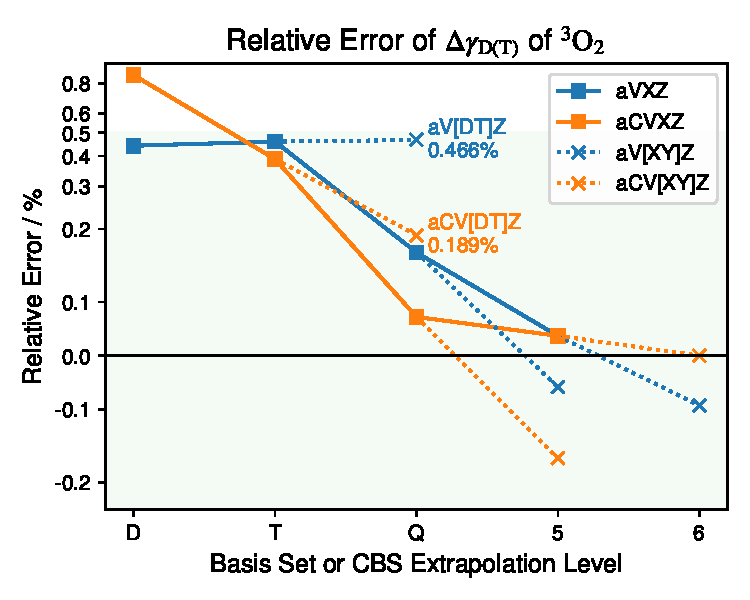
\includegraphics[width=0.5\textwidth]{assets/O2-aniso.pdf}
    \caption[$\symup{\Delta} \gamma_\textsf{D(T)}$ 对体系 \ce{^3O2} 计算结果的基组收敛趋势]{$\symup{\Delta} \gamma_\textsf{D(T)}$ 对体系 \ce{^3O2} 计算结果的基组收敛趋势。}
    \label{fig.O2-aniso}
\end{figure}

\textbf{\ce{^3SO} 的基组收敛性。}收敛情况如图 \ref{fig.SO-aniso} 所示。该体系是非常具有挑战性的体系,因此其基组误差或 CBS 外推误差都不是非常有规律,且误差较大。尽管如此,aCV5Z、aV5Z 或 aV[Q5]Z 的误差都远小于 0.5\%,因此使用这些大小的基组估计 \ce{^3SO} 的异性极化率,仍然是可以接受的。

\begin{figure}[ht]
    \centering
    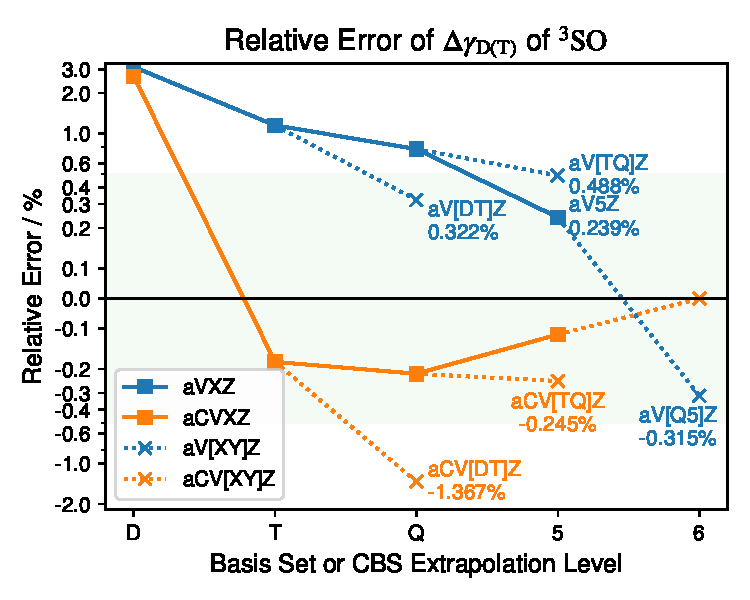
\includegraphics[width=0.5\textwidth]{assets/SO-aniso.pdf}
    \caption[$\symup{\Delta} \gamma_\textsf{D(T)}$ 对体系 \ce{^3SO} 计算结果的基组收敛趋势]{$\symup{\Delta} \gamma_\textsf{D(T)}$ 对体系 \ce{^3SO} 计算结果的基组收敛趋势。}
    \label{fig.SO-aniso}
\end{figure}

\textbf{\ce{HCHS} 的基组收敛性。}收敛情况如图 \ref{fig.HCHS-aniso} 所示。可以发现该体系下,基组收敛趋势在 QZ (4-$\zeta$) 处出现了剧烈的转折。因此,更昂贵的 aV[TQ]Z、aCV[TQ]Z 外推结果不如 aV[DT]Z、aCV[DT]Z,也不如基组 aVQZ、aCVQZ。

\begin{figure}[ht]
    \centering
    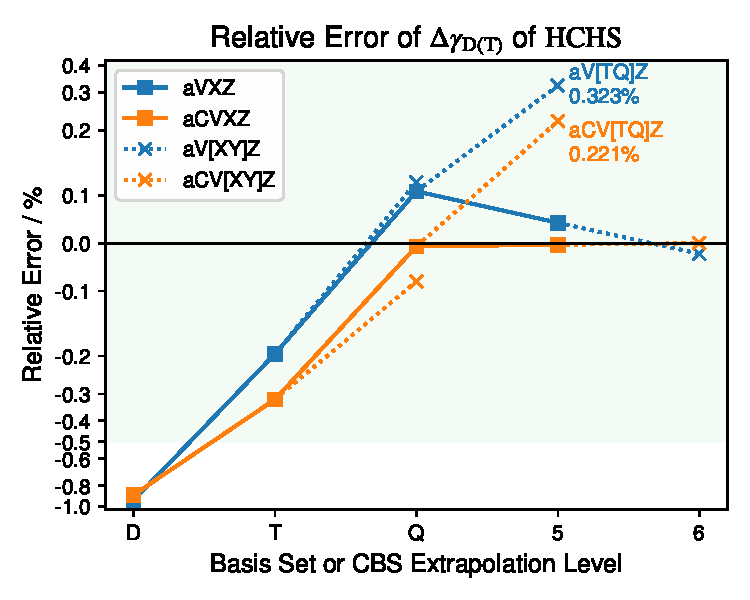
\includegraphics[width=0.5\textwidth]{assets/HCHS-aniso.pdf}
    \caption[$\symup{\Delta} \gamma_\textsf{D(T)}$ 对体系 \ce{HCHS} 计算结果的基组收敛趋势]{$\symup{\Delta} \gamma_\textsf{D(T)}$ 对体系 \ce{HCHS} 计算结果的基组收敛趋势。}
    \label{fig.HCHS-aniso}
\end{figure}

\textbf{\ce{Cl2} 的基组收敛性。}收敛情况如图 \ref{fig.Cl2-aniso} 所示。该体系与 \ce{HCHS} 体系的情况类似,在 QZ (4-$\zeta$) 处 aV$X$Z 的收敛趋势发生了转折;对于 aCV$X$Z 而言,其收敛趋势也与式 (\ref{eq.cbs.zeta3}) 有一定偏离。因此,更昂贵的 CBS 外推,未必比更低等级的外推的误差更小。

\begin{figure}[ht]
    \centering
    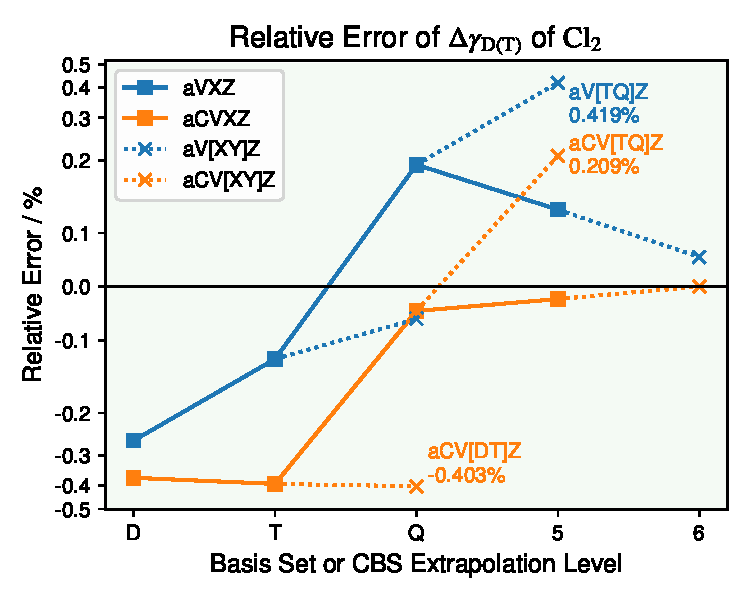
\includegraphics[width=0.5\textwidth]{assets/Cl2-aniso.pdf}
    \caption[$\symup{\Delta} \gamma_\textsf{D(T)}$ 对体系 \ce{Cl2} 计算结果的基组收敛趋势]{$\symup{\Delta} \gamma_\textsf{D(T)}$ 对体系 \ce{Cl2} 计算结果的基组收敛趋势。}
    \label{fig.Cl2-aniso}
\end{figure}

\newpage

\subsection{更新后的 HR46 与 T144 极化率参考值}

更新后的 HR46 与 T144 极化率参考值数据列于表 \ref{tab.5.s1}, \ref{tab.5.s2}, \ref{tab.5.s3}, \ref{tab.5.s4}。对于同性极化率,HF 方法极化率以 $\alpha_{\textsf{HF}/\text{aCV5Z}}$ 计算,MP2 方法极化率以 $\alpha_{\textsf{HF}/\text{aCV5Z}} + \symup{\Delta} \alpha_{\textsf{(2)}/\text{aCV[Q5]Z}}$ 计算。CCSD 与 CCSD(T) 依照不同分子大小划分不同的子集;每个子集使用其对应的 FPA 模型。对于异性极化率 $\gamma$ 同样如此。上述记号在表 \ref{tab.5.1} 中定义,FPA 模型的计算方式在式 (\ref{eq.5.fpa-alpha}, \ref{eq.5.fpa-gamma}) 定义,数据子集及其对应 FPA 模型在表 \ref{tab.5.4} 给出。

\begingroup
\setlength{\LTleft}{-20cm plus -1fill}
\setlength{\LTright}{\LTleft}

\begin{longtable}{lcd{1.4}d{1.4}d{1.4}d{1.4}}
    \caption[HR46 数据集子集分割情况与同性极化率 $\alpha$ 参考值]{HR46 数据集子集分割情况与同性极化率 $\alpha$ 参考值。极化率单位为 $\textrm{\AA}{}^{3}$。}
    \label{tab.5.s1}
    \\ \toprule
    体系名称 & 子集 & \multicolumn{1}{c}{SCF} & \multicolumn{1}{c}{MP2} & \multicolumn{1}{c}{CCSD} & \multicolumn{1}{c}{CCSD(T)} \\ \midrule
    \endfirsthead
    \caption[]{(续表)}
    \\ \toprule
    体系名称 & 子集 & \multicolumn{1}{c}{SCF} & \multicolumn{1}{c}{MP2} & \multicolumn{1}{c}{CCSD} & \multicolumn{1}{c}{CCSD(T)} \\ \midrule
    \endhead
    \bottomrule
    \endfoot
    %
    dibromine                        & I   & 6.4900  & 6.4892  & 6.4491  & 6.4860  \\
    dichlorine                       & I   & 4.4524  & 4.5128  & 4.4623  & 4.4946  \\
    dinitrogen                       & I   & 1.7382  & 1.7147  & 1.7320  & 1.7513  \\
    dioxygen                         & I   & 1.6997  & 1.3631  & 1.5725  & 1.5753  \\
    carbon   monoxide                & I   & 1.8369  & 1.9518  & 1.9143  & 1.9359  \\
    nitrogen   monoxide              & I   & 1.5974  & 1.5638  & 1.6560  & 1.6735  \\
    sulfur   monoxide                & I   & 3.4772  & 3.2412  & 3.4134  & 3.4233  \\
    carbon   dioxide                 & I   & 2.3679  & 2.6457  & 2.5508  & 2.5893  \\
    sulfur   dioxide                 & I   & 3.6122  & 3.9235  & 3.8081  & 3.8691  \\
    ethene                           & II  & 4.1149  & 3.9894  & 3.9264  & 3.9390  \\
    propane                          & II  & 5.6906  & 5.9136  & 5.7929  & 5.8568  \\
    buta-1,3-diene                   & II  & 8.3973  & 8.0088  & 7.8624  & 7.8881  \\
    2-methylprop-1-ene               & III & 7.5161  & 7.6041  & 7.4537  & 7.5203  \\
    pent-1-ene                       & III & 9.2785  & 9.4332  & 9.2363  & 9.3295  \\
    water                            & I   & 1.2655  & 1.4334  & 1.3756  & 1.4088  \\
    methanol                         & II  & 2.9061  & 3.0965  & 3.0207  & 3.0665  \\
    ethanol                          & II  & 4.5863  & 4.8614  & 4.7448  & 4.8150  \\
    methyl   formate                 & II  & 4.5929  & 4.9915  & 4.8558  & 4.9483  \\
    methyl   acetate                 & III & 6.2409  & 6.7178  & 6.5543  & 6.6706  \\
    propan-2-one                     & II  & 5.7652  & 6.1113  & 5.9725  & 6.0643  \\
    acetaldehyde                     & II  & 4.1546  & 4.4051  & 4.3053  & 4.3719  \\
    acetic acid                      & II  & 4.5962  & 5.0041  & 4.8659  & 4.9581  \\
    methoxymethane                   & II  & 4.6047  & 4.8892  & 4.7710  & 4.8458  \\
    \textit{N}-methylacetamide       & III & 6.9306  & 7.5082  & 7.3063  & 7.4476  \\
    (methylsulfanyl)methane          & II  & 6.9614  & 7.2041  & 7.0491  & 7.1292  \\
    (methanesulfonyl)methane         & III & 7.1953  & 7.8804  & 7.6318  & 7.7896  \\
    fluoromethane                    & II  & 2.3370  & 2.4742  & 2.4242  & 2.4567  \\
    phosphorus   trihydride          & I   & 4.3558  & 4.4377  & 4.3741  & 4.4036  \\
    hydrogen   sulfide               & I   & 3.5212  & 3.6039  & 3.5383  & 3.5702  \\
    silicon   tetrahydride           & I   & 4.3649  & 4.5242  & 4.5235  & 4.5578  \\
    ammonia                          & I   & 1.9113  & 2.0973  & 2.0285  & 2.0685  \\
    \textit{N}-methylmethanamine     & III & 5.2406  & 5.5599  & 5.4220  & 5.5068  \\
    \textit{N},\textit{N}-dimethylmethanamine & III & 6.9422  & 7.4313  & 7.2232  & 7.3550  \\
    acetonitrile                     & II  & 4.2244  & 4.2594  & 4.2240  & 4.2729  \\
    1\textit{H}-imidazole                     & III & 6.9643  & 7.1519  & 7.0127  & 7.1068  \\
    1\textit{H}-pyrrole                       & III & 7.8658  & 7.9808  & 7.8205  & 7.9031  \\
    1\textit{H}-pyrazole                      & II  & 6.9567  & 7.1563  & 7.0109  & 7.0930  \\
    furan                            & III & 7.0133  & 7.0682  & 6.9398  & 7.0109  \\
    thiophene                        & III & 9.2525  & 9.3688  & 9.1874  & 9.2705  \\
    pyridine                         & III & 9.1427  & 9.3139  & 9.0928  & 9.1601  \\
    phenol                           & III & 10.5747 & 10.9115 & 10.6252 & 10.7336 \\
    chlorobenzene                    & III & 11.9811 & 12.2430 & 11.9528 & 12.0564 \\
    fluorobenzene                    & III & 9.8705  & 10.0900 & 9.8465  & 9.9259  \\
    toluene                          & III & 11.7837 & 12.0204 & 11.7230 & 11.8159 \\
    benzene                          & III & 9.9989  & 10.0978 & 9.8569  & 9.9148  \\
    6-amino-1\textit{H}-pyrimidin-2-one       & III & 10.4008 & 11.4939 & 11.1193 & 11.3642
\end{longtable}

\begin{longtable}{lcd{2.5}d{2.5}d{2.5}d{2.5}}
    \caption[HR46 数据集子集分割情况与异性极化率 $\gamma$ 参考值]{HR46 数据集子集分割情况与异性极化率 $\gamma$ 参考值。极化率单位为 $\textrm{\AA}{}^{3}$。}
    \label{tab.5.s2}
    \\ \toprule
    体系名称 & 子集 & \multicolumn{1}{c}{SCF} & \multicolumn{1}{c}{MP2} & \multicolumn{1}{c}{CCSD} & \multicolumn{1}{c}{CCSD(T)} \\ \midrule
    \endfirsthead
    \caption[]{(续表)}
    \\ \toprule
    体系名称 & 子集 & \multicolumn{1}{c}{SCF} & \multicolumn{1}{c}{MP2} & \multicolumn{1}{c}{CCSD} & \multicolumn{1}{c}{CCSD(T)} \\ \midrule
    \endhead
    \bottomrule
    \endfoot
    %
    dichlorine                 & I   & 2.7190 & 2.4874 & 2.5427 & 2.5095 \\
    dinitrogen                 & I   & 0.7973 & 0.6358 & 0.7005 & 0.7012 \\
    dioxygen                   & I   & 1.5982 & 0.5794 & 1.1208 & 1.0813 \\
    carbon monoxide            & I   & 0.4857 & 0.5526 & 0.5493 & 0.5434 \\
    nitrogen monoxide          & I   & 0.8249 & 0.5248 & 0.7895 & 0.7723 \\
    sulfur monoxide            & I   & 1.8707 & 1.0157 & 1.5435 & 1.4718 \\
    carbon dioxide             & I   & 1.7571 & 2.1739 & 2.0571 & 2.0811 \\
    sulfur dioxide             & I   & 1.9327 & 2.1051 & 2.1060 & 2.1031 \\
    ethene                     & II  & 1.8922 & 1.5721 & 1.6393 & 1.6048 \\
    propane                    & II  & 0.7927 & 0.9269 & 0.8662 & 0.8950 \\
    buta-1,3-diene             & II  & 7.2789 & 6.0403 & 6.0481 & 5.9747 \\
    2-methylprop-1-ene         & III & 2.8287 & 2.5764 & 2.6044 & 2.5912 \\
    pent-1-ene                 & III & 3.7292 & 3.6171 & 3.5668 & 3.5949 \\
    water                      & I   & 0.1695 & 0.0632 & 0.1023 & 0.0872 \\
    methanol                   & II  & 0.4482 & 0.4795 & 0.4617 & 0.4720 \\
    ethanol                    & II  & 0.7372 & 0.8046 & 0.7825 & 0.8016 \\
    methyl formate             & II  & 1.4593 & 1.7977 & 1.7097 & 1.7794 \\
    methyl acetate             & III & 1.8505 & 2.2655 & 2.1414 & 2.2385 \\
    propan-2-one               & II  & 1.5086 & 1.7432 & 1.6743 & 1.7240 \\
    acetaldehyde               & II  & 1.3982 & 1.5450 & 1.5216 & 1.5506 \\
    acetic acid                & II  & 1.4093 & 1.6702 & 1.6053 & 1.6546 \\
    methoxymethane             & II  & 0.9770 & 1.0219 & 1.0029 & 1.0206 \\
    \textit{N}-methylacetamide          & III & 2.2239 & 2.7445 & 2.5950 & 2.7153 \\
    (methylsulfanyl)methane    & II  & 1.7291 & 1.7873 & 1.7575 & 1.7726 \\
    (methanesulfonyl)methane   & III & 0.5736 & 0.5728 & 0.5576 & 0.5733 \\
    fluoromethane              & II  & 0.1733 & 0.2295 & 0.2187 & 0.2277 \\
    phosphorus trihydride      & I   & 0.1692 & 0.2459 & 0.2035 & 0.2219 \\
    hydrogen sulfide           & I   & 0.0614 & 0.0860 & 0.0548 & 0.0680 \\
    silicon tetrahydride       & I   & 0.0000 & 0.0000 & 0.0000 & 0.0002 \\
    ammonia                    & I   & 0.0805 & 0.2707 & 0.2107 & 0.2435 \\
    \textit{N}-methylmethanamine        & III & 0.8821 & 0.9574 & 0.9163 & 0.9400 \\
    \textit{N},\textit{N}-dimethylmethanamine    & III & 0.7967 & 0.6456 & 0.6744 & 0.6425 \\
    acetonitrile               & II  & 2.1822 & 2.1620 & 2.1730 & 2.2075 \\
    1\textit{H}-imidazole               & III & 3.0288 & 3.2599 & 3.1950 & 3.2601 \\
    1\textit{H}-pyrrole                 & III & 3.2098 & 3.3974 & 3.3673 & 3.4125 \\
    1\textit{H}-pyrazole                & II  & 3.0035 & 3.2064 & 3.1592 & 3.2039 \\
    furan                      & III & 2.8699 & 3.0339 & 2.9829 & 3.0349 \\
    thiophene                  & III & 4.1626 & 4.3174 & 4.2843 & 4.3248 \\
    pyridine                   & III & 4.7026 & 5.0514 & 4.8613 & 4.9108 \\
    phenol                     & III & 5.6312 & 6.1789 & 5.9511 & 6.0444 \\
    chlorobenzene              & III & 6.9954 & 7.4551 & 7.1968 & 7.2903 \\
    fluorobenzene              & III & 5.0733 & 5.4818 & 5.2945 & 5.3554 \\
    toluene                    & III & 5.9811 & 6.4286 & 6.1810 & 6.2542 \\
    benzene                    & III & 4.9828 & 5.3181 & 5.1358 & 5.1779 \\
    6-amino-1\textit{H}-pyrimidin-2-one & III & 6.5310 & 7.7469 & 7.4832 & 7.6917
\end{longtable}

\begin{longtable}{rlcd{2.5}d{2.5}d{2.5}d{2.5}}
    \caption[T144 数据集子集分割情况与同性极化率 $\alpha$ 参考值]{T144 数据集子集分割情况与同性极化率 $\alpha$ 参考值。极化率单位为 $\textrm{\AA}{}^{3}$。}
    \label{tab.5.s3}
    \\ \toprule
    编号 & 体系名称 & 子集 & \multicolumn{1}{c}{SCF} & \multicolumn{1}{c}{MP2} & \multicolumn{1}{c}{CCSD} & \multicolumn{1}{c}{CCSD(T)} \\ \midrule
    \endfirsthead
    \caption[]{(续表)}
    \\ \toprule
    编号 & 体系名称 & 子集 & \multicolumn{1}{c}{SCF} & \multicolumn{1}{c}{MP2} & \multicolumn{1}{c}{CCSD} & \multicolumn{1}{c}{CCSD(T)} \\ \midrule
    \endhead
    \bottomrule
    \endfoot
    %
    56   & azidoethene                                            & II & 8.0681  & 8.0481  & 7.9500  & 8.0009  \\
    93   & 2-bromoacetonitrile                                    & I  & 7.2968  & 7.3427  & 7.2654  & 7.3479  \\
    97   & bromo(chloro)methane                                   & I  & 7.2828  & 7.4452  & 7.3325  & 7.4129  \\
    103  & bromoethene                                            & I  & 7.0622  & 7.0289  & 6.9263  & 6.9812  \\
    112  & buta-1,3-diyne-1,4-diol                                & II & 8.5401  & 8.8206  & 8.5898  & 8.7817  \\
    117  & butanenitrile                                          & II & 7.6474  & 7.8507  & 7.7283  & 7.8279  \\
    119  & buta-1,2,3-triene                                      & I  & 9.1418  & 8.5124  & 8.3872  & 8.3605  \\
    129  & methyl   carbonochloridodithioate                      & II & 12.3741 & 12.9106 & 12.6625 & 12.8474 \\
    142  & chloroethene                                           & I  & 5.9901  & 5.9911  & 5.8877  & 5.9363  \\
    158  & carbononitridic fluoride                               & I  & 2.5791  & 2.6437  & 2.6187  & 2.6595  \\
    159  & 2-cyanoacetyl isocyanate                               & II & 8.8338  & 9.5315  & 9.2963  & 9.4780  \\
    205  & buta-1,3-diyne                                         & I  & 7.1606  & 6.9381  & 6.8048  & 6.9068  \\
    213  & dibromo(chloro)methane                                 & I  & 10.2793 & 10.5245 & 10.3618 & 10.4915 \\
    223  & propanedinitrile                                       & I  & 6.0934  & 6.0881  & 6.0605  & 6.1413  \\
    245  & dimethyl sulfite                                       & II & 8.0667  & 8.7769  & 8.5317  & 8.7123  \\
    256  & (methylsulfonyl)methane                                & II & 7.3477  & 8.0408  & 7.7855  & 7.9460  \\
    257  & (methylsulfinyl)methane                                & II & 7.4069  & 7.9788  & 7.7279  & 7.8804  \\
    267  & ethanedithioamide                                      & II & 12.9133 & 13.7325 & 13.3992 & 13.6181 \\
    276  & (\textit{E})-penta-1,3-diene                           & II & 10.3663 & 10.0859 & 9.8877  & 9.9486  \\
    281  & (\textit{E})-but-2-enenitrile                          & II & 8.1061  & 8.0503  & 7.9438  & 8.0205  \\
    282  & (\textit{E})-2-chlorobut-2-ene                         & II & 9.5183  & 9.6839  & 9.5228  & 9.6219  \\
    287  & (\textit{E})-3-bromoprop-2-enoic   acid                & II & 9.7101  & 10.1143 & 9.8953  & 10.0540 \\
    306  & ethanethioamide                                        & II & 8.4689  & 8.9883  & 8.7663  & 8.8979  \\
    318  & ethoxyethene                                           & II & 8.4125  & 8.6995  & 8.4876  & 8.6005  \\
    332  & ethyl formate                                          & II & 6.3714  & 6.8685  & 6.6948  & 6.8161  \\
    336  & ethyl nitrate                                          & II & 7.0244  & 7.5315  & 7.3915  & 7.5135  \\
    342  & bis(ethynyloxy)methane                                 & II & 9.6739  & 9.9363  & 9.7043  & 9.8805  \\
    346  & bis(ethynylthio)methane                                & II & 14.7861 & 15.0609 & 14.7025 & 14.9522 \\
    351  & fluoroethane                                           & I  & 4.0310  & 4.2471  & 4.1594  & 4.2149  \\
    353  & fluoromethane                                          & I  & 2.3577  & 2.4952  & 2.4449  & 2.4774  \\
    361  & fulvene                                                & II & 10.9909 & 10.5843 & 10.4118 & 10.4503 \\
    381  & hexachloroethane                                       & II & 15.1760 & 15.8485 & 15.5460 & 15.7799 \\
    390  & hexa-1,3,5-triyne                                      & II & 12.1906 & 11.9368 & 11.5251 & 11.8120 \\
    393  & hydroperoxyethyne                                      & I  & 5.3880  & 5.3928  & 5.3003  & 5.4010  \\
    397  & disulfanediyldimethanol                                & II & 11.2293 & 11.9416 & 11.6400 & 11.8538 \\
    399  & hydroperoxymethanol                                    & I  & 4.4564  & 4.7569  & 4.6538  & 4.7523  \\
    425  & 1,2-thiazole                                           & II & 8.4584  & 8.6724  & 8.4893  & 8.5804  \\
    438  & furan-2,5-dione                                        & II & 7.6615  & 7.9792  & 7.8434  & 7.9672  \\
    445  & methanesulfonyl chloride                               & II & 7.8783  & 8.5530  & 8.3135  & 8.4710  \\
    460  & methyl \textit{N}-cyanocarbamodithioate                & II & 13.7169 & 14.4935 & 14.1680 & 14.4192 \\
    470  & methyl hypochlorite                                    & I  & 5.0676  & 5.2069  & 5.1345  & 5.2022  \\
    489  & 1-methylsulfinylethane                                 & II & 9.0847  & 9.7314  & 9.4479  & 9.6239  \\
    529  & \textit{N}-methylacetamide                             & II & 7.0137  & 7.6100  & 7.3991  & 7.5450  \\
    533  & \textit{N}-methylmethanesulfinamide                    & II & 8.6404  & 9.3453  & 9.0530  & 9.2446  \\
    556  & \textit{N},\textit{N}-dimethylformamide                & II & 7.0933  & 7.7056  & 7.4895  & 7.6360  \\
    580  & \textit{O}-ethynylhydroxylamine                        & I  & 5.7154  & 5.8418  & 5.7111  & 5.8104  \\
    599  & oxirane                                                & I  & 4.0025  & 4.2108  & 4.1059  & 4.1631  \\
    617  & penta-2,4-diynal                                       & II & 9.8822  & 9.8627  & 9.6189  & 9.8365  \\
    654  & prop-2-ynoyl chloride                                  & I  & 7.5324  & 7.7513  & 7.5997  & 7.7394  \\
    655  & prop-2-ynoyl fluoride                                  & I  & 5.4285  & 5.5537  & 5.4644  & 5.5567  \\
    670  & prop-2-ynenitrile                                      & I  & 5.8466  & 5.6951  & 5.6323  & 5.7180  \\
    710  & \textit{S}-methyl methanethioate                       & II & 7.2153  & 7.6850  & 7.4985  & 7.6319  \\
    722  & 2-sulfanylacetyl chloride                              & II & 9.0295  & 9.5355  & 9.3199  & 9.4742  \\
    753  & 1,3-thiazole                                           & II & 8.4287  & 8.6663  & 8.4865  & 8.5972  \\
    757  & ethanethial                                            & I  & 7.0464  & 7.0397  & 6.9622  & 7.0034  \\
    761  & [(thiocyanatomethyl)sulfanyl]ethyne                    & II & 13.4609 & 13.7605 & 13.4900 & 13.7194 \\
    762  & methanethione                                          & I  & 5.1572  & 4.9828  & 4.9647  & 4.9708  \\
    765  & 1\textit{H}-1$\lambda^4$-thiophen-1-one                & II & 9.7138  & 10.1194 & 9.8264  & 9.9955  \\
    767  & thiocarbonyl dichloride                                & I  & 9.1897  & 9.3734  & 9.2637  & 9.3726  \\
    768  & hydrazinecarbothioamide                                & II & 9.2341  & 10.1227 & 9.7994  & 10.0360 \\
    769  & thiourea                                               & I  & 7.9223  & 8.6554  & 8.3855  & 8.5711  \\
    818  & (\textit{Z})-1,2-dichloroethene                        & I  & 7.8436  & 7.9339  & 7.7965  & 7.8760  \\
    820  & (\textit{Z})-1,2,3-trifluoroprop-1-ene                 & II & 5.7100  & 5.9439  & 5.8223  & 5.8996  \\
    833  & (\textit{Z})-pent-3-en-1-yne                           & II & 9.2484  & 9.0613  & 8.9102  & 8.9953  \\
    841  & 1,3-difluoro-1\textit{H}-pyrrole                       & II & 7.9289  & 8.1413  & 8.0149  & 8.1175  \\
    843  & 1-azido-2-chloroethane                                 & II & 9.0258  & 9.3774  & 9.2214  & 9.3307  \\
    846  & 2-bromobutanedinitrile                                 & II & 10.8725 & 10.9959 & 10.8776 & 11.0264 \\
    847  & 1-bromo-2-chloroethane                                 & II & 9.2207  & 9.4728  & 9.3333  & 9.4403  \\
    852  & 1-bromo-1-isothiocyanatoethane                         & II & 13.3650 & 14.0961 & 13.7610 & 13.9381 \\
    884  & 2,2-difluoropropanenitrile                             & II & 5.9373  & 6.1845  & 6.0951  & 6.1957  \\
    886  & (\textit{E})-3-fluoroprop-2-enenitrile                 & I  & 6.1625  & 6.1588  & 6.0773  & 6.1462  \\
    890  & 1-(difluoroamino)ethanol                               & II & 6.1333  & 6.5536  & 6.4275  & 6.5399  \\
    909  & buta-1,3-diyn-1-ol                                     & I  & 7.8920  & 7.9329  & 7.7375  & 7.8867  \\
    936  & methyl ethanimidothioate                               & II & 9.6535  & 10.1400 & 9.9096  & 10.0704 \\
    969  & 1,1-dichloro-2,2,2-trifluoroethane                     & II & 7.8580  & 8.3185  & 8.1659  & 8.2925  \\
    974  & 1,1-difluoro-1-hydroperoxyethane                       & II & 5.4458  & 5.8127  & 5.7046  & 5.8095  \\
    976  & 1,1-difluoro-2-isothiocyanatoethane                    & II & 10.0764 & 10.7629 & 10.5105 & 10.6370 \\
    987  & 1,1-dicyanatoethene                                    & II & 8.9566  & 9.2798  & 9.1240  & 9.2930  \\
    989  & 1,1,1-tribromoethane                                   & II & 13.0953 & 13.3895 & 13.2096 & 13.3674 \\
    998  & 1,1,1,2-tetrafluoroethane                              & II & 4.1213  & 4.5140  & 4.4110  & 4.4960  \\
    1003 & 1,1,2-trifluoroprop-1-ene                              & II & 5.7094  & 5.9726  & 5.8474  & 5.9257  \\
    1014 & buta-1,2-diene                                         & II & 7.9390  & 7.8233  & 7.6909  & 7.7361  \\
    1019 & 2,3-dichloropropanenitrile                             & II & 9.8049  & 10.0548 & 9.9154  & 10.0496 \\
    1032 & 1,2-difluoroethane                                     & I  & 4.0301  & 4.3017  & 4.2070  & 4.2722  \\
    1046 & propa-1,2-diene-1,3-dione                              & I  & 6.4283  & 7.0533  & 6.8867  & 6.9090  \\
    1047 & 1\textit{H}-1$\lambda^4$,2-thiazole-1-one              & II & 8.8947  & 9.3850  & 9.1036  & 9.2774  \\
    1048 & 1,2-thiazole-3-carbonitrile                            & II & 10.8429 & 11.0316 & 10.8418 & 10.9910 \\
    1049 & 1,2-thiazole-3(2\textit{H})-thione                     & II & 13.0692 & 13.8705 & 13.4717 & 13.7146 \\
    1074 & 1,2,4-triazine                                         & II & 7.6665  & 7.8929  & 7.7170  & 7.7946  \\
    1085 & 1,2,6-oxathiazine                                      & II & 9.3056  & 9.5888  & 9.3624  & 9.5070  \\
    1108 & 1,3-oxazolidine-2,5-dithione                           & II & 13.5497 & 14.3977 & 14.1122 & 14.3525 \\
    1109 & penta-1,3-diyne                                        & II & 9.3074  & 9.2102  & 9.0067  & 9.1558  \\
    1115 & 1,3-thiazolidine-2-thione                              & II & 12.5292 & 13.3536 & 12.9860 & 13.2082 \\
    1117 & 1,3,2-oxathiazole                                      & II & 7.8181  & 8.1037  & 7.9049  & 8.0268  \\
    1119 & 1,3,4-thiadiazolidine-2,5-dithione                     & II & 15.8784 & 17.1398 & 16.6929 & 17.0311 \\
    1135 & 1,4-dithiane                                           & II & 12.4528 & 12.9714 & 12.6666 & 12.8429 \\
    1149 & 1\textit{H}-pyrazole                                   & II & 6.9689  & 7.1826  & 7.0300  & 7.1148  \\
    1193 & 2-bromoethen-1-one                                     & I  & 6.9926  & 7.2590  & 7.1121  & 7.1885  \\
    1194 & 2-bromoethen-1-imine                                   & I  & 8.1901  & 8.3309  & 8.2145  & 8.2978  \\
    1197 & (\textit{E})-1-bromo-2-fluoroethene                    & I  & 6.9199  & 6.9971  & 6.8852  & 6.9556  \\
    1207 & but-2-ynedinitrile                                     & I  & 8.9700  & 8.7923  & 8.6391  & 8.8477  \\
    1209 & 2-chlorobut-1-ene                                      & II & 9.3442  & 9.5424  & 9.3658  & 9.4678  \\
    1241 & 2-fluoroethen-1-imine                                  & I  & 5.1020  & 5.2137  & 5.1225  & 5.1757  \\
    1250 & 2-hydroxypropanenitrile                                & II & 6.4869  & 6.7327  & 6.6193  & 6.7246  \\
    1251 & imidazolidine-2-thione                                 & II & 10.7170 & 11.5987 & 11.2548 & 11.4863 \\
    1256 & 2-isothiocyanato-1,3-thiazole                          & II & 15.8391 & 16.8419 & 16.2918 & 16.5693 \\
    1314 & propane-2-thiol                                        & II & 8.7104  & 9.0672  & 8.8582  & 8.9712  \\
    1315 & propan-2-imine                                         & II & 6.6737  & 6.9218  & 6.7881  & 6.8782  \\
    1332 & 2-sulfanylideneethanethioamide                         & II & 11.6246 & 11.8245 & 11.6573 & 11.8209 \\
    1344 & 2,2-difluoro-1,3-dithiolane                            & II & 10.6713 & 11.2593 & 10.9829 & 11.1622 \\
    1361 & 2,3-dihydro-1\textit{H}-1$\lambda^4$,2-thiazole-1-one  & II & 9.2049  & 9.7749  & 9.4863  & 9.6704  \\
    1367 & 2,3-dihydro-1\textit{H}-1$\lambda^4$-thiophene-1-one   & II & 9.8566  & 10.3624 & 10.0723 & 10.2447 \\
    1378 & furo[2,3-d][1,3,2]dioxathiole                          & II & 10.0941 & 10.5835 & 10.3082 & 10.4969 \\
    1382 & 2,3,3-trifluoroprop-1-ene                              & II & 5.7730  & 6.0059  & 5.8784  & 5.9601  \\
    1391 & 2,4-difluoropyrimidine                                 & II & 8.1794  & 8.7344  & 8.4864  & 8.6035  \\
    1395 & hexa-2,4-diyne                                         & II & 11.4822 & 11.5157 & 11.2544 & 11.4516 \\
    1396 & hexa-2,4-diynedial                                     & II & 12.8186 & 13.0567 & 12.6733 & 13.0325 \\
    1406 & 2,5-dihydro-1\textit{H}-1$\lambda^4$,2-thiazole-1-one  & II & 9.2475  & 9.8457  & 9.5380  & 9.7216  \\
    1408 & 2,5-dihydrofuran                                       & II & 7.2055  & 7.3836  & 7.2298  & 7.3175  \\
    1409 & 2,5-dihydro-1\textit{H}-1$\lambda^4$-thiophene-1-one   & II & 9.8554  & 10.3411 & 10.0543 & 10.2215 \\
    1428 & 2\textit{H}-1$\lambda^6$-thiete-1,1-dione              & II & 8.2438  & 8.8283  & 8.5558  & 8.7200  \\
    1429 & 3-(chloromethyl)-1,2,5-thiadiazole                     & II & 11.6396 & 12.0209 & 11.7950 & 11.9491 \\
    1438 & 3-aminopropanenitrile                                  & II & 7.1847  & 7.4993  & 7.3542  & 7.4788  \\
    1444 & 3-(bromomethyl)-1,2,4-oxadiazole                       & II & 10.2889 & 10.7045 & 10.4790 & 10.6294 \\
    1455 & 3-chloropyridine                                       & II & 11.2136 & 11.5580 & 11.2813 & 11.4020 \\
    1457 & 3-diazopropanenitrile                                  & II & 8.3412  & 8.3755  & 8.3193  & 8.3839  \\
    1475 & 3-iminopropa-1,2-dien-1-one                            & I  & 7.8060  & 8.4914  & 8.3267  & 8.3565  \\
    1479 & 3-isothiocyanatopropanenitrile                         & II & 12.2123 & 12.7762 & 12.5147 & 12.6606 \\
    1502 & 3-methylsulfanylprop-2-ynenitrile                      & II & 11.5791 & 11.7857 & 11.5113 & 11.7397 \\
    1563 & 4-bromo-1,3-dioxolan-2-one                             & II & 9.2897  & 9.8983  & 9.6963  & 9.8671  \\
    1564 & 4-bromo-1,3-thiazole                                   & II & 11.6057 & 11.9537 & 11.7275 & 11.8887 \\
    1588 & 4-imino-1,3-thiazolidine-2-thione                      & II & 13.8771 & 14.8442 & 14.4674 & 14.7453 \\
    1603 & 4-sulfanyl-1,3-thiazole-5-carbonitrile                 & II & 14.0608 & 14.5223 & 14.1907 & 14.4132 \\
    1604 & 4-sulfanylidene-1,3-thiazolidin-2-one                  & II & 12.6924 & 13.6283 & 13.2860 & 13.5354 \\
    1607 & pyrimidin-4(3\textit{H})-one                           & II & 9.0415  & 9.6122  & 9.3568  & 9.5029  \\
    1610 & 4,5-dihydro-1\textit{H}-1$\lambda^4$,2-thiazole-1-one  & II & 9.1176  & 9.7145  & 9.4378  & 9.6180  \\
    1617 & 5-amino-1,3-thiazole-2(3\textit{H})-thione             & II & 14.0661 & 15.2320 & 14.7001 & 15.0229 \\
    1619 & 5-bromo-1\textit{H}-pyrazole                           & II & 10.0029 & 10.3130 & 10.1260 & 10.2600 \\
    1622 & 5-chloro-4-methyl-1,2,3-thiadiazole                    & II & 11.6141 & 12.0519 & 11.8421 & 12.0225 \\
    1625 & 4,5-dihydrothiophen-2-ol                               & II & 10.1478 & 10.5655 & 10.2979 & 10.4468 \\
    1626 & 5-hydroxypenta-2,4-diynoic   acid                      & II & 11.1002 & 11.6959 & 11.3217 & 11.6427 \\
    1630 & 5-methyl-1\textit{H}-tetrazole                         & II & 7.2026  & 7.5802  & 7.4283  & 7.5513  \\
    1633 & 5,5,5-trichloropenta-1,3-diyne                         & II & 15.8092 & 16.1354 & 15.7009 & 16.0388 \\
    1634 & 5,5,5-trifluoropenta-1,3-diyne                         & II & 9.2386  & 9.3951  & 9.1692  & 9.3657 
\end{longtable}

\begin{longtable}{rlcd{2.5}d{2.5}d{2.5}d{2.5}}
    \caption[T144 数据集子集分割情况与异性极化率 $\gamma$ 参考值]{T144 数据集子集分割情况与异性极化率 $\gamma$ 参考值。极化率单位为 $\text{\AA}{}^{3}$。}
    \label{tab.5.s4}
    \\ \toprule
    编号 & 体系名称 & 子集 & \multicolumn{1}{c}{SCF} & \multicolumn{1}{c}{MP2} & \multicolumn{1}{c}{CCSD} & \multicolumn{1}{c}{CCSD(T)} \\ \midrule
    \endfirsthead
    \caption[]{(续表)}
    \\ \toprule
    编号 & 体系名称 & 子集 & \multicolumn{1}{c}{SCF} & \multicolumn{1}{c}{MP2} & \multicolumn{1}{c}{CCSD} & \multicolumn{1}{c}{CCSD(T)} \\ \midrule
    \endhead
    \bottomrule
    \endfoot
    %
    56   & azidoethene                                            & II & 9.0731  & 8.6158  & 8.7252  & 8.6987  \\
    93   & 2-bromoacetonitrile                                    & I  & 3.6425  & 3.5412  & 3.5362  & 3.5862  \\
    97   & bromo(chloro)methane                                   & I  & 3.3412  & 3.3591  & 3.3379  & 3.3703  \\
    103  & bromoethene                                            & I  & 4.0723  & 3.8011  & 3.8248  & 3.8267  \\
    112  & buta-1,3-diyne-1,4-diol                                & II & 9.9425  & 10.6544 & 10.2490 & 10.6018 \\
    117  & butanenitrile                                          & II & 3.2723  & 3.4013  & 3.3454  & 3.4255  \\
    119  & buta-1,2,3-triene                                      & I  & 11.7541 & 9.8291  & 9.9289  & 9.7312  \\
    129  & methyl   carbonochloridodithioate                      & II & 7.7193  & 8.1661  & 8.1086  & 8.2186  \\
    142  & chloroethene                                           & I  & 3.4061  & 3.1953  & 3.2037  & 3.2065  \\
    158  & carbononitridic fluoride                               & I  & 1.4134  & 1.5022  & 1.5107  & 1.5416  \\
    159  & 2-cyanoacetyl isocyanate                               & II & 6.4594  & 7.6808  & 7.3308  & 7.5931  \\
    205  & buta-1,3-diyne                                         & I  & 7.8797  & 7.6295  & 7.4217  & 7.6127  \\
    213  & dibromo(chloro)methane                                 & I  & 3.7141  & 3.7329  & 3.7047  & 3.7527  \\
    223  & propanedinitrile                                       & I  & 3.0672  & 2.9728  & 3.0142  & 3.0742  \\
    245  & dimethyl sulfite                                       & II & 1.6412  & 1.7220  & 1.7415  & 1.7886  \\
    256  & (methylsulfonyl)methane                                & II & 0.7146  & 0.7079  & 0.6906  & 0.7062  \\
    257  & (methylsulfinyl)methane                                & II & 1.6271  & 1.7384  & 1.7118  & 1.7412  \\
    267  & ethanedithioamide                                      & II & 8.3814  & 9.4550  & 9.1653  & 9.2964  \\
    276  & (\textit{E})-penta-1,3-diene                           & II & 8.8735  & 7.7352  & 7.6475  & 7.6187  \\
    281  & (\textit{E})-but-2-enenitrile                          & II & 6.0461  & 5.7416  & 5.6893  & 5.7534  \\
    282  & (\textit{E})-2-chlorobut-2-ene                         & II & 4.6671  & 4.4595  & 4.4460  & 4.4698  \\
    287  & (\textit{E})-3-bromoprop-2-enoic   acid                & II & 7.0320  & 7.2889  & 7.0696  & 7.2391  \\
    306  & ethanethioamide                                        & II & 3.9062  & 4.5858  & 4.4282  & 4.5065  \\
    318  & ethoxyethene                                           & II & 4.1670  & 4.3383  & 4.2637  & 4.3280  \\
    332  & ethyl formate                                          & II & 2.1231  & 2.6423  & 2.5081  & 2.6157  \\
    336  & ethyl nitrate                                          & II & 3.0870  & 3.5831  & 3.4750  & 3.6043  \\
    342  & bis(ethynyloxy)methane                                 & II & 7.2402  & 7.7849  & 7.5804  & 7.7901  \\
    346  & bis(ethynylthio)methane                                & II & 8.7181  & 9.0806  & 8.7840  & 9.0676  \\
    351  & fluoroethane                                           & I  & 0.3800  & 0.4911  & 0.4597  & 0.4804  \\
    353  & fluoromethane                                          & I  & 0.1808  & 0.2363  & 0.2264  & 0.2351  \\
    361  & fulvene                                                & II & 8.1178  & 6.8562  & 7.0831  & 6.9683  \\
    381  & hexachloroethane                                       & II & 1.1960  & 1.0268  & 1.0820  & 1.0397  \\
    390  & hexa-1,3,5-triyne                                      & II & 17.9903 & 17.7693 & 16.8033 & 17.5058 \\
    393  & hydroperoxyethyne                                      & I  & 4.2888  & 4.2237  & 4.1517  & 4.2803  \\
    397  & disulfanediyldimethanol                                & II & 3.4922  & 3.7334  & 3.6947  & 3.7811  \\
    399  & hydroperoxymethanol                                    & I  & 2.0249  & 1.7510  & 1.8334  & 1.8584  \\
    425  & 1,2-thiazole                                           & II & 4.1444  & 4.2860  & 4.2387  & 4.2778  \\
    438  & furan-2,5-dione                                        & II & 5.7093  & 5.6961  & 5.7788  & 5.8467  \\
    445  & methanesulfonyl chloride                               & II & 2.2935  & 2.2404  & 2.2799  & 2.2743  \\
    460  & methyl \textit{N}-cyanocarbamodithioate                & II & 8.7533  & 9.5074  & 9.3599  & 9.5078  \\
    470  & methyl hypochlorite                                    & I  & 2.5226  & 2.2198  & 2.3270  & 2.3262  \\
    489  & 1-methylsulfinylethane                                 & II & 2.1786  & 2.4050  & 2.3470  & 2.3998  \\
    529  & \textit{N}-methylacetamide                             & II & 2.3645  & 2.9188  & 2.7541  & 2.8849  \\
    533  & \textit{N}-methylmethanesulfinamide                    & II & 2.7020  & 2.7910  & 2.7702  & 2.8153  \\
    556  & \textit{N},\textit{N}-dimethylformamide                & II & 2.5649  & 3.1859  & 3.0465  & 3.1593  \\
    580  & \textit{O}-ethynylhydroxylamine                        & I  & 4.0172  & 4.1430  & 4.0510  & 4.1465  \\
    599  & oxirane                                                & I  & 0.9355  & 0.8405  & 0.8533  & 0.8450  \\
    617  & penta-2,4-diynal                                       & II & 11.9632 & 12.0000 & 11.5237 & 11.9866 \\
    654  & prop-2-ynoyl chloride                                  & I  & 4.3710  & 4.5509  & 4.4069  & 4.5601  \\
    655  & prop-2-ynoyl fluoride                                  & I  & 3.7781  & 3.8118  & 3.7643  & 3.8570  \\
    670  & prop-2-ynenitrile                                      & I  & 6.1079  & 5.8668  & 5.7879  & 5.9364  \\
    710  & \textit{S}-methyl methanethioate                       & II & 3.5629  & 4.0737  & 3.9756  & 4.0964  \\
    722  & 2-sulfanylacetyl chloride                              & II & 2.4576  & 2.8864  & 2.7237  & 2.8517  \\
    753  & 1,3-thiazole                                           & II & 3.8270  & 4.1157  & 4.0428  & 4.1287  \\
    757  & ethanethial                                            & I  & 3.7674  & 3.5795  & 3.6497  & 3.6148  \\
    761  & [(thiocyanatomethyl)sulfanyl]ethyne                    & II & 7.2041  & 7.5472  & 7.3619  & 7.6168  \\
    762  & methanethione                                          & I  & 2.7321  & 2.3328  & 2.4730  & 2.4160  \\
    765  & 1\textit{H}-1$\lambda^4$-thiophen-1-one                & II & 4.9482  & 5.1080  & 5.0778  & 5.1744  \\
    767  & thiocarbonyl dichloride                                & I  & 4.9610  & 4.8797  & 4.9861  & 5.0148  \\
    768  & hydrazinecarbothioamide                                & II & 4.3557  & 5.3873  & 5.0986  & 5.3227  \\
    769  & thiourea                                               & I  & 3.5380  & 4.3938  & 4.1938  & 4.3436  \\
    818  & (\textit{Z})-1,2-dichloroethene                        & I  & 4.1809  & 3.9204  & 3.9412  & 3.9522  \\
    820  & (\textit{Z})-1,2,3-trifluoroprop-1-ene                 & II & 2.5233  & 2.4284  & 2.4161  & 2.4230  \\
    833  & (\textit{Z})-pent-3-en-1-yne                           & II & 6.2591  & 5.6432  & 5.6352  & 5.6774  \\
    841  & 1,3-difluoro-1\textit{H}-pyrrole                       & II & 3.8139  & 3.9878  & 3.9892  & 4.0481  \\
    843  & 1-azido-2-chloroethane                                 & II & 4.4204  & 4.4567  & 4.4699  & 4.4887  \\
    846  & 2-bromobutanedinitrile                                 & II & 4.6691  & 4.6066  & 4.6060  & 4.7123  \\
    847  & 1-bromo-2-chloroethane                                 & II & 5.2783  & 5.3225  & 5.2545  & 5.3014  \\
    852  & 1-bromo-1-isothiocyanatoethane                         & II & 7.9990  & 9.4639  & 8.9572  & 9.1764  \\
    884  & 2,2-difluoropropanenitrile                             & II & 2.0026  & 1.9376  & 1.9501  & 1.9935  \\
    886  & (\textit{E})-3-fluoroprop-2-enenitrile                 & I  & 4.5583  & 4.4504  & 4.4112  & 4.4781  \\
    890  & 1-(difluoroamino)ethanol                               & II & 1.1542  & 1.1299  & 1.1400  & 1.1488  \\
    909  & buta-1,3-diyn-1-ol                                     & I  & 8.9885  & 9.2526  & 8.9138  & 9.1899  \\
    936  & methyl ethanimidothioate                               & II & 3.6717  & 4.1478  & 3.9863  & 4.1208  \\
    969  & 1,1-dichloro-2,2,2-trifluoroethane                     & II & 2.2838  & 2.3349  & 2.3083  & 2.3366  \\
    974  & 1,1-difluoro-1-hydroperoxyethane                       & II & 1.3828  & 1.1155  & 1.1855  & 1.1905  \\
    976  & 1,1-difluoro-2-isothiocyanatoethane                    & II & 7.9835  & 9.1909  & 8.8447  & 8.9626  \\
    987  & 1,1-dicyanatoethene                                    & II & 5.6561  & 6.2953  & 6.1784  & 6.4119  \\
    989  & 1,1,1-tribromoethane                                   & II & 2.7988  & 2.5637  & 2.6302  & 2.6266  \\
    998  & 1,1,1,2-tetrafluoroethane                              & II & 0.2218  & 0.2816  & 0.2741  & 0.2863  \\
    1003 & 1,1,2-trifluoroprop-1-ene                              & II & 2.6259  & 2.6048  & 2.5612  & 2.5738  \\
    1014 & buta-1,2-diene                                         & II & 6.1978  & 5.4739  & 5.5806  & 5.5220  \\
    1019 & 2,3-dichloropropanenitrile                             & II & 4.0346  & 4.0314  & 4.0078  & 4.0845  \\
    1032 & 1,2-difluoroethane                                     & I  & 0.4463  & 0.5661  & 0.5490  & 0.5691  \\
    1046 & propa-1,2-diene-1,3-dione                              & I  & 8.4200  & 10.0774 & 9.7239  & 9.7215  \\
    1047 & 1\textit{H}-1$\lambda^4$,2-thiazole-1-one              & II & 4.7596  & 4.8937  & 4.8590  & 4.9543  \\
    1048 & 1,2-thiazole-3-carbonitrile                            & II & 7.6912  & 7.7750  & 7.6756  & 7.8248  \\
    1049 & 1,2-thiazole-3(2\textit{H})-thione                     & II & 10.1167 & 11.3540 & 11.0223 & 11.3010 \\
    1074 & 1,2,4-triazine                                         & II & 4.1325  & 4.3739  & 4.2079  & 4.2511  \\
    1085 & 1,2,6-oxathiazine                                      & II & 4.5076  & 4.4532  & 4.4485  & 4.5053  \\
    1108 & 1,3-oxazolidine-2,5-dithione                           & II & 9.6147  & 11.1574 & 10.8877 & 11.2000 \\
    1109 & penta-1,3-diyne                                        & II & 10.1751 & 10.1084 & 9.7589  & 10.0441 \\
    1115 & 1,3-thiazolidine-2-thione                              & II & 6.8454  & 7.8516  & 7.5650  & 7.7246  \\
    1117 & 1,3,2-oxathiazole                                      & II & 3.0202  & 2.9296  & 2.9440  & 2.9684  \\
    1119 & 1,3,4-thiadiazolidine-2,5-dithione                     & II & 13.7164 & 15.8813 & 15.4527 & 15.8977 \\
    1135 & 1,4-dithiane                                           & II & 3.1501  & 3.2124  & 3.1678  & 3.1903  \\
    1149 & 1\textit{H}-pyrazole                                   & II & 3.0220  & 3.2282  & 3.1833  & 3.2292  \\
    1193 & 2-bromoethen-1-one                                     & I  & 4.4117  & 4.6599  & 4.6067  & 4.6339  \\
    1194 & 2-bromoethen-1-imine                                   & I  & 6.2491  & 6.1608  & 6.2144  & 6.2373  \\
    1197 & (\textit{E})-1-bromo-2-fluoroethene                    & I  & 3.9495  & 3.8801  & 3.8614  & 3.8900  \\
    1207 & but-2-ynedinitrile                                     & I  & 12.3779 & 12.0385 & 11.6677 & 12.1430 \\
    1209 & 2-chlorobut-1-ene                                      & II & 3.4936  & 3.5407  & 3.4989  & 3.5431  \\
    1241 & 2-fluoroethen-1-imine                                  & I  & 4.3178  & 4.1732  & 4.2256  & 4.2165  \\
    1250 & 2-hydroxypropanenitrile                                & II & 2.1167  & 2.1163  & 2.1189  & 2.1662  \\
    1251 & imidazolidine-2-thione                                 & II & 5.2401  & 6.4372  & 6.0973  & 6.3156  \\
    1256 & 2-isothiocyanato-1,3-thiazole                          & II & 14.8286 & 17.1918 & 16.1087 & 16.5742 \\
    1314 & propane-2-thiol                                        & II & 1.8879  & 1.9744  & 1.9005  & 1.9299  \\
    1315 & propan-2-imine                                         & II & 2.2221  & 2.2208  & 2.2153  & 2.2410  \\
    1332 & 2-sulfanylideneethanethioamide                         & II & 6.2950  & 6.4178  & 6.3851  & 6.5537  \\
    1344 & 2,2-difluoro-1,3-dithiolane                            & II & 2.7544  & 2.9425  & 2.8500  & 2.9057  \\
    1361 & 2,3-dihydro-1\textit{H}-1$\lambda^4$,2-thiazole-1-one  & II & 3.3202  & 3.2537  & 3.2676  & 3.3107  \\
    1367 & 2,3-dihydro-1\textit{H}-1$\lambda^4$-thiophene-1-one   & II & 3.2685  & 3.2156  & 3.2152  & 3.2546  \\
    1378 & furo[2,3-d][1,3,2]dioxathiole                          & II & 5.6189  & 6.1868  & 5.9187  & 6.1305  \\
    1382 & 2,3,3-trifluoroprop-1-ene                              & II & 2.4047  & 2.1797  & 2.1968  & 2.1854  \\
    1391 & 2,4-difluoropyrimidine                                 & II & 4.4064  & 5.0519  & 4.8244  & 4.9226  \\
    1395 & hexa-2,4-diyne                                         & II & 12.6359 & 12.7676 & 12.2833 & 12.6709 \\
    1396 & hexa-2,4-diynedial                                     & II & 16.5087 & 17.0234 & 16.1807 & 16.9963 \\
    1406 & 2,5-dihydro-1\textit{H}-1$\lambda^4$,2-thiazole-1-one  & II & 2.6259  & 2.6543  & 2.6392  & 2.6810  \\
    1408 & 2,5-dihydrofuran                                       & II & 2.9072  & 2.7180  & 2.7488  & 2.7560  \\
    1409 & 2,5-dihydro-1\textit{H}-1$\lambda^4$-thiophene-1-one   & II & 2.7397  & 2.6692  & 2.6710  & 2.6939  \\
    1428 & 2\textit{H}-1$\lambda^6$-thiete-1,1-dione              & II & 2.2527  & 2.2485  & 2.2189  & 2.2567  \\
    1429 & 3-(chloromethyl)-1,2,5-thiadiazole                     & II & 6.1811  & 6.2069  & 6.1646  & 6.2423  \\
    1438 & 3-aminopropanenitrile                                  & II & 3.2125  & 3.4024  & 3.3329  & 3.4318  \\
    1444 & 3-(bromomethyl)-1,2,4-oxadiazole                       & II & 4.3883  & 4.6944  & 4.5368  & 4.6530  \\
    1455 & 3-chloropyridine                                       & II & 6.8858  & 7.3693  & 7.1062  & 7.2211  \\
    1457 & 3-diazopropanenitrile                                  & II & 5.5477  & 5.1981  & 5.3767  & 5.3377  \\
    1475 & 3-iminopropa-1,2-dien-1-one                            & I  & 10.8652 & 12.6525 & 12.3641 & 12.3519 \\
    1479 & 3-isothiocyanatopropanenitrile                         & II & 10.9068 & 12.1904 & 11.7782 & 11.9730 \\
    1502 & 3-methylsulfanylprop-2-ynenitrile                      & II & 11.6158 & 11.9443 & 11.4973 & 11.9394 \\
    1563 & 4-bromo-1,3-dioxolan-2-one                             & II & 3.3623  & 3.7350  & 3.6647  & 3.7634  \\
    1564 & 4-bromo-1,3-thiazole                                   & II & 7.0300  & 7.3579  & 7.2362  & 7.3678  \\
    1588 & 4-imino-1,3-thiazolidine-2-thione                      & II & 9.4901  & 10.8260 & 10.5266 & 10.7957 \\
    1603 & 4-sulfanyl-1,3-thiazole-5-carbonitrile                 & II & 8.0174  & 8.4353  & 8.2021  & 8.3909  \\
    1604 & 4-sulfanylidene-1,3-thiazolidin-2-one                  & II & 7.9894  & 9.2594  & 8.9990  & 9.2323  \\
    1607 & pyrimidin-4(3\textit{H})-one                           & II & 5.3676  & 5.9803  & 5.8206  & 5.9367  \\
    1610 & 4,5-dihydro-1\textit{H}-1$\lambda^4$,2-thiazole-1-one  & II & 3.1473  & 3.1886  & 3.1767  & 3.2325  \\
    1617 & 5-amino-1,3-thiazole-2(3\textit{H})-thione             & II & 9.6404  & 11.9763 & 11.1351 & 11.6176 \\
    1619 & 5-bromo-1\textit{H}-pyrazole                           & II & 5.7034  & 6.0555  & 5.9057  & 6.0242  \\
    1622 & 5-chloro-4-methyl-1,2,3-thiadiazole                    & II & 5.7511  & 6.1593  & 6.0223  & 6.1760  \\
    1625 & 4,5-dihydrothiophen-2-ol                               & II & 3.7383  & 3.8346  & 3.7932  & 3.8374  \\
    1626 & 5-hydroxypenta-2,4-diynoic   acid                      & II & 12.7329 & 13.7212 & 13.0318 & 13.6367 \\
    1630 & 5-methyl-1\textit{H}-tetrazole                         & II & 3.2079  & 3.6111  & 3.4466  & 3.5492  \\
    1633 & 5,5,5-trichloropenta-1,3-diyne                         & II & 10.9431 & 11.2261 & 10.5173 & 11.0520 \\
    1634 & 5,5,5-trifluoropenta-1,3-diyne                         & II & 9.5362  & 9.6309  & 9.2565  & 9.5907 
\end{longtable}

\endgroup
